\documentclass[10pt, aspectratio=169, handout]{beamer}

% ============================================
% PACKAGES
% ============================================
\usetheme{metropolis}
\usepackage{appendixnumberbeamer}

\usepackage[utf8]{inputenc}
\usepackage[T1]{fontenc}
\usepackage{amsmath,amssymb,amsfonts}
\usepackage{graphicx}
\usepackage{tikz}
\usetikzlibrary{arrows.meta,positioning,decorations.pathmorphing,calc,shapes.geometric}
\usepackage{booktabs}
\usepackage[scale=2]{ccicons}
\usepackage{xcolor}
\usepackage[table]{xcolor}
% Colore ottanio chiaro per backup slides
\definecolor{ottanio}{RGB}{64,160,180}
\usepackage{float}
\usepackage{pgfplots}
\usepgfplotslibrary{dateplot}
\usepackage{subcaption}
\pgfplotsset{compat=1.18}
\usepackage{FiraMono}
\usepackage{FiraSans}
\usepackage{xspace}
\usepackage{appendixnumberbeamer}
\newcommand{\themename}{\textbf{\textsc{metropolis}}\xspace}


% Sfondo bianco
\setbeamercolor{background canvas}{bg=white}

% ============================================
% THEME SETTINGS
% ============================================

\setbeamertemplate{navigation symbols}{}
\setbeamerfont{author}{size=\normalsize}
\setbeamerfont{institute}{size=\normalsize}
\setbeamerfont{date}{size=\normalsize}
\setbeamertemplate{footline}[frame number]

% ============================================
% TITLE INFO
% ============================================
\title{Simulation of LiteBIRD Instrumental Noise with the LBS Framework}
\author{Giulia Giommoni}
\institute{}
\date{\footnotesize{Anno Accademico 2024--2025}}

% ============================================
\begin{document}
% ============================================



%-------------------------------------------
% SLIDE 0: TITOLO
%-------------------------------------------
{%
\setbeamertemplate{footline}{}
\begin{frame}[noframenumbering]
  \begin{center}
    
\includegraphics[height=3cm]{logo.jpg}\\[0.4cm]
    {\Large\textbf{Simulation of LiteBIRD Instrumental Noise with the LBS Framework}}\\[0.8cm]
    \begin{columns}[T]
      \begin{column}{0.45\textwidth}
        \raggedright
        Candidata:\\
        Giulia Giommoni
      \end{column}
      \begin{column}{0.45\textwidth}
        \raggedleft
        Relatore:\\
        Prof.~Maurizio Tomasi
      \end{column}
    \end{columns}
    \vspace{0.8cm}
    {\footnotesize Anno Accademico 2024--2025}
  \end{center}
\end{frame}
}





%-------------------------------------------
% SLIDE 1: LA MISSIONE LITEBIRD
%-------------------------------------------
\begin{frame}{Missione LiteBIRD}

  \begin{columns}[c]
    
    % --- COLONNA DI SINISTRA: TESTO ---
    \begin{column}{0.45\textwidth}
      \footnotesize 
      
      \textit{\textbf{L}ite satellite for the study of \textbf{B}-mode polarization and \textbf{I}nflation from cosmic background \textbf{R}adiation \textbf{D}etection}
      
      \vspace{0.6cm}
      
      \metroset{block=transparent}
      \begin{description}
        \item[\textbf{Missione:}] Mappatura della polarizzazione della CMB.
        
        \vspace{0.2cm}
        
        \item[\textbf{Obiettivo:}] Ricerca dei modi B primordiali.
        
        \vspace{0.2cm}
        
        \item[\textbf{Target:}] Evidenza diretta dell'inflazione.
      \end{description}
      
    \end{column}

    % --- COLONNA DI DESTRA: IMMAGINE ---
    \begin{column}{0.45\textwidth}
      \centering
      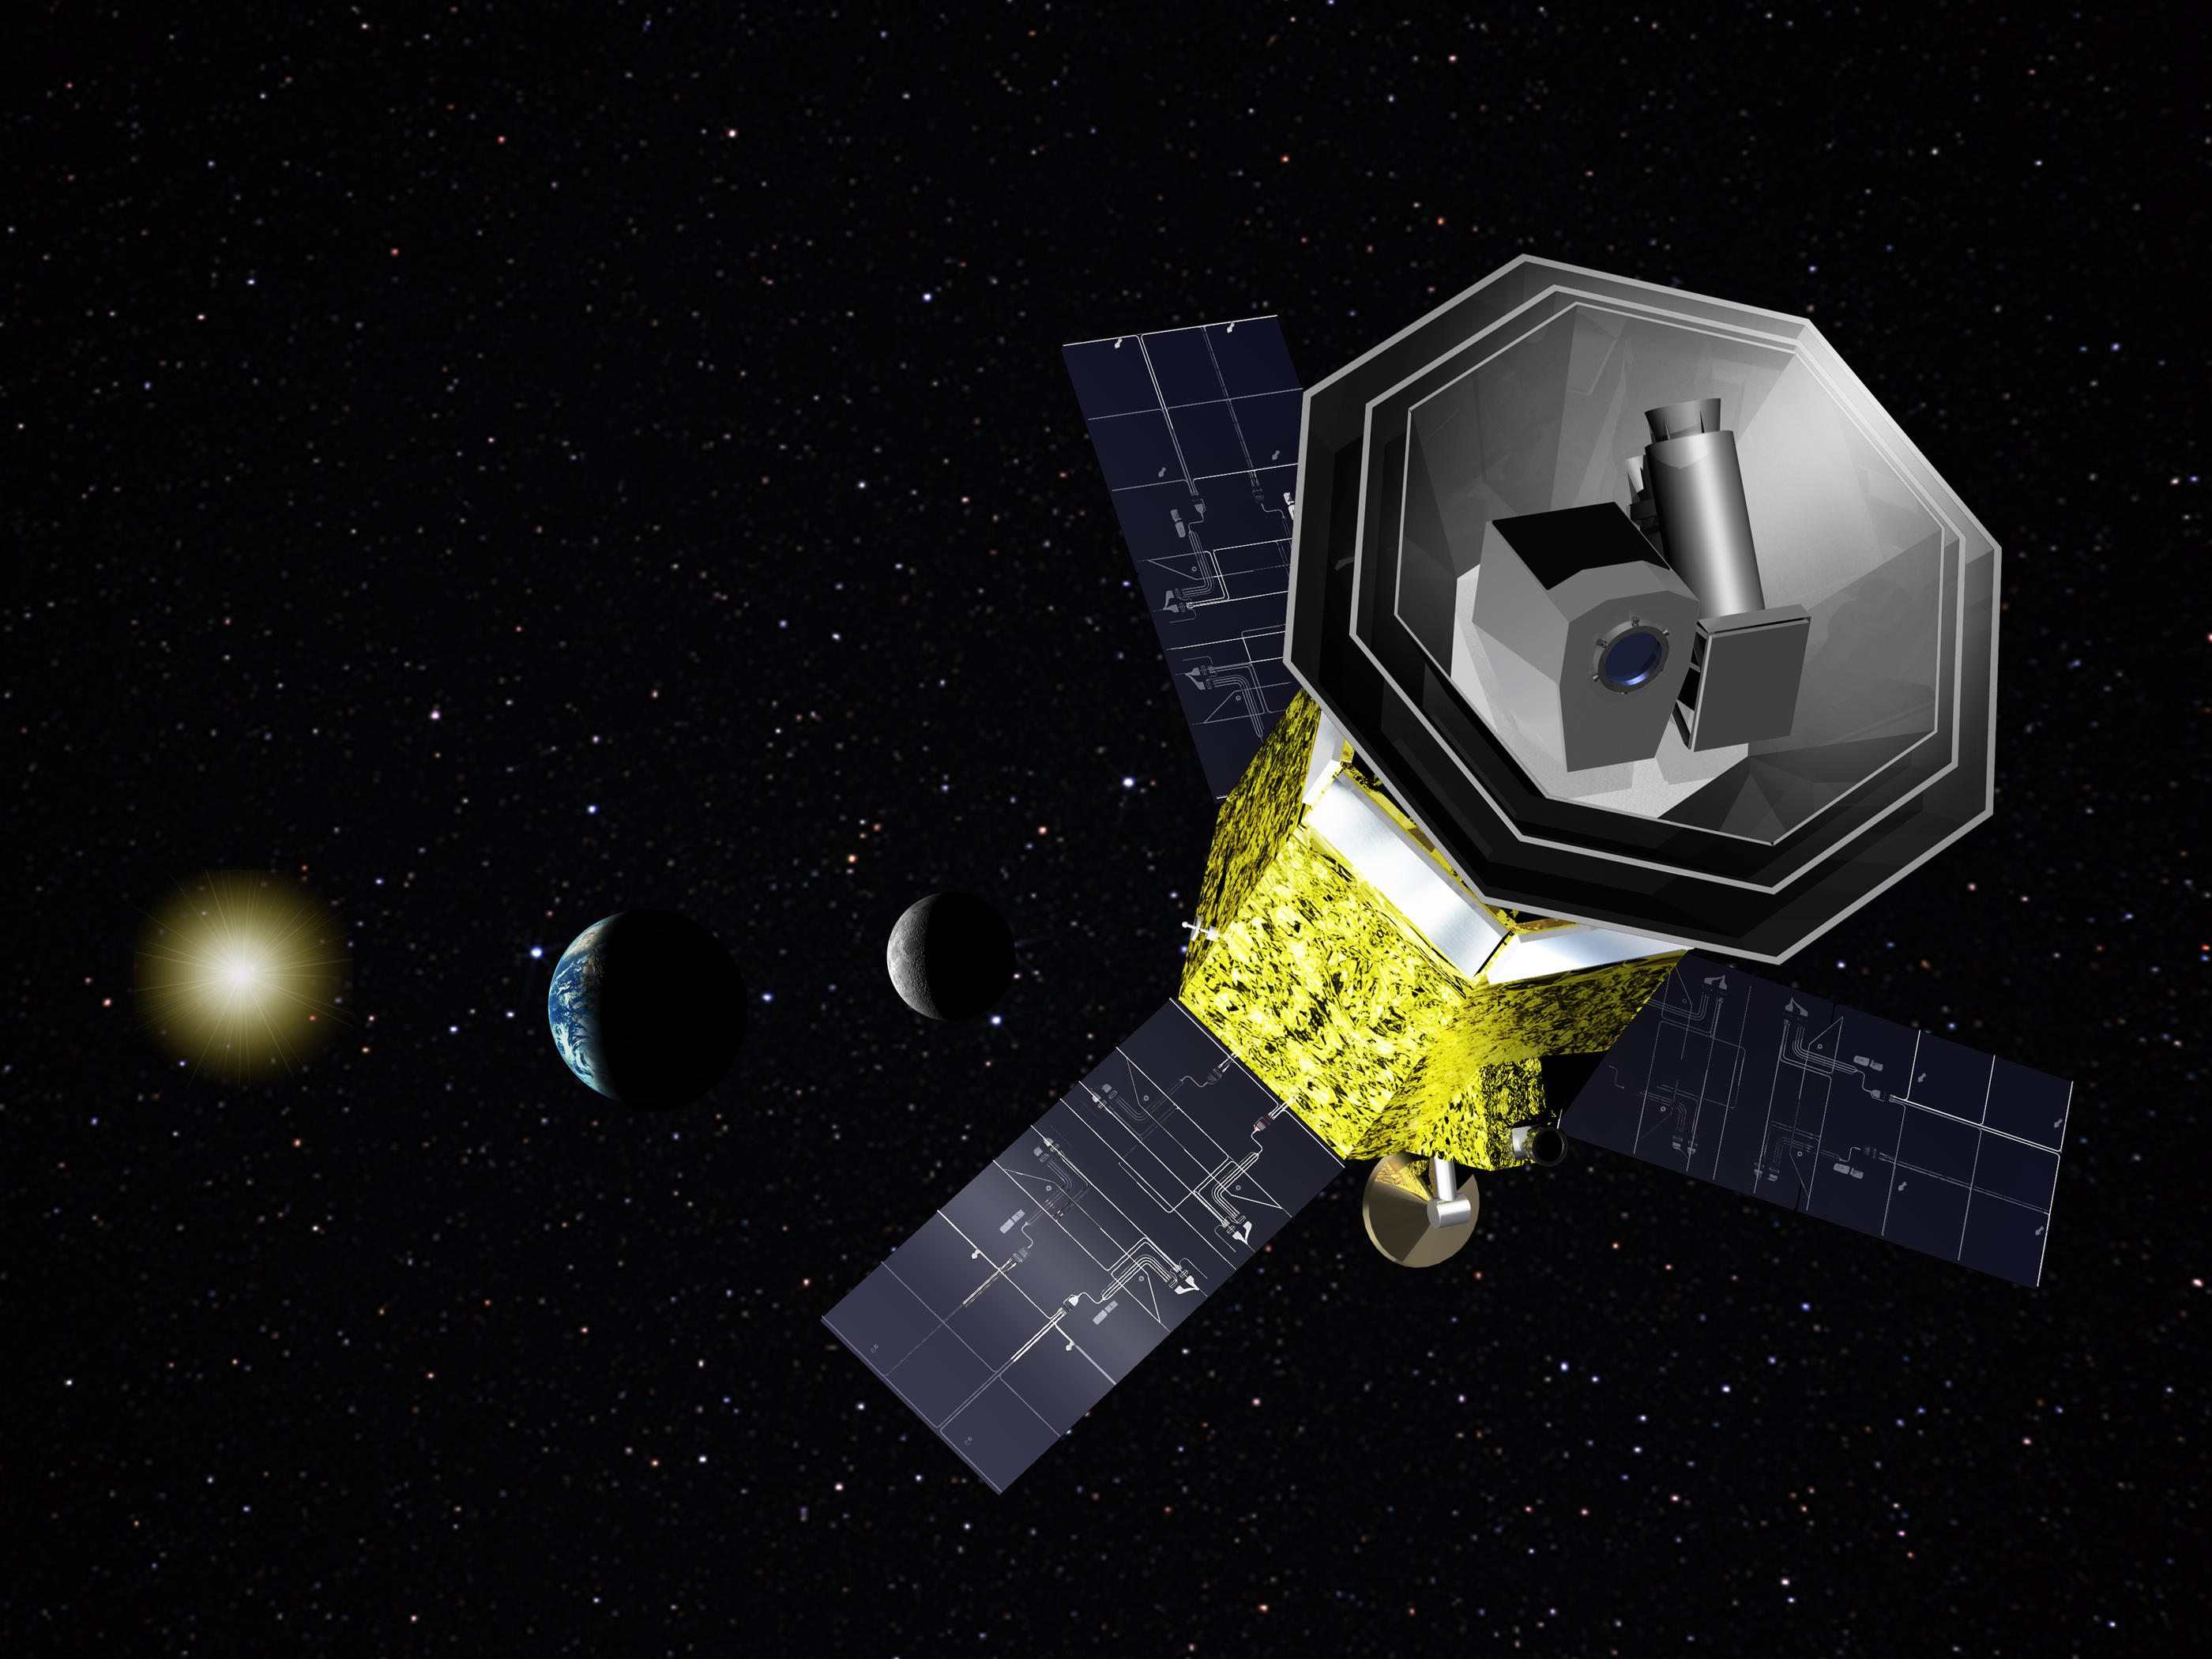
\includegraphics[width=\linewidth]{1_LiteBIRD.jpg}
    \end{column}

  \end{columns}
\end{frame}





%-------------------------------------------
% SLIDE 2: MODI B E INFLAZIONE
%-------------------------------------------
\begin{frame}{Modi B e Inflazione}

  \begin{columns}[c] 
  
    % --- COLONNA DI SINISTRA: FISICA E OBIETTIVO ---
    \begin{column}{0.5\textwidth}
      \metroset{block=transparent}
      \begin{block}{L'impronta dell'Inflazione}
        \footnotesize
        \begin{itemize}
          \item Onde gravitazionali primordiali $\rightarrow$ \textbf{Modi B}.
          \item Segnale estremamente debole: $\mathbf{\ll 1\,\mu K}$.
        \end{itemize}
      \end{block}

      \vspace{0.4cm}

      \begin{block}{La Sfida Sperimentale}
        \footnotesize
        \begin{itemize}
          \item Criticità: \textbf{effetti sistematici strumentali}.
          \item Il rumore può mascherare il segnale cosmologico.
        \end{itemize}
      \end{block}
      
      \vspace{0.4cm} 
      
      \centering
      \scriptsize\textit{Necessità di simulare il rumore strumentale.}
    \end{column}

    % --- COLONNA DI DESTRA: IMMAGINE EVOLUTIVA ---
    \begin{column}{0.5\textwidth}
      \centering
      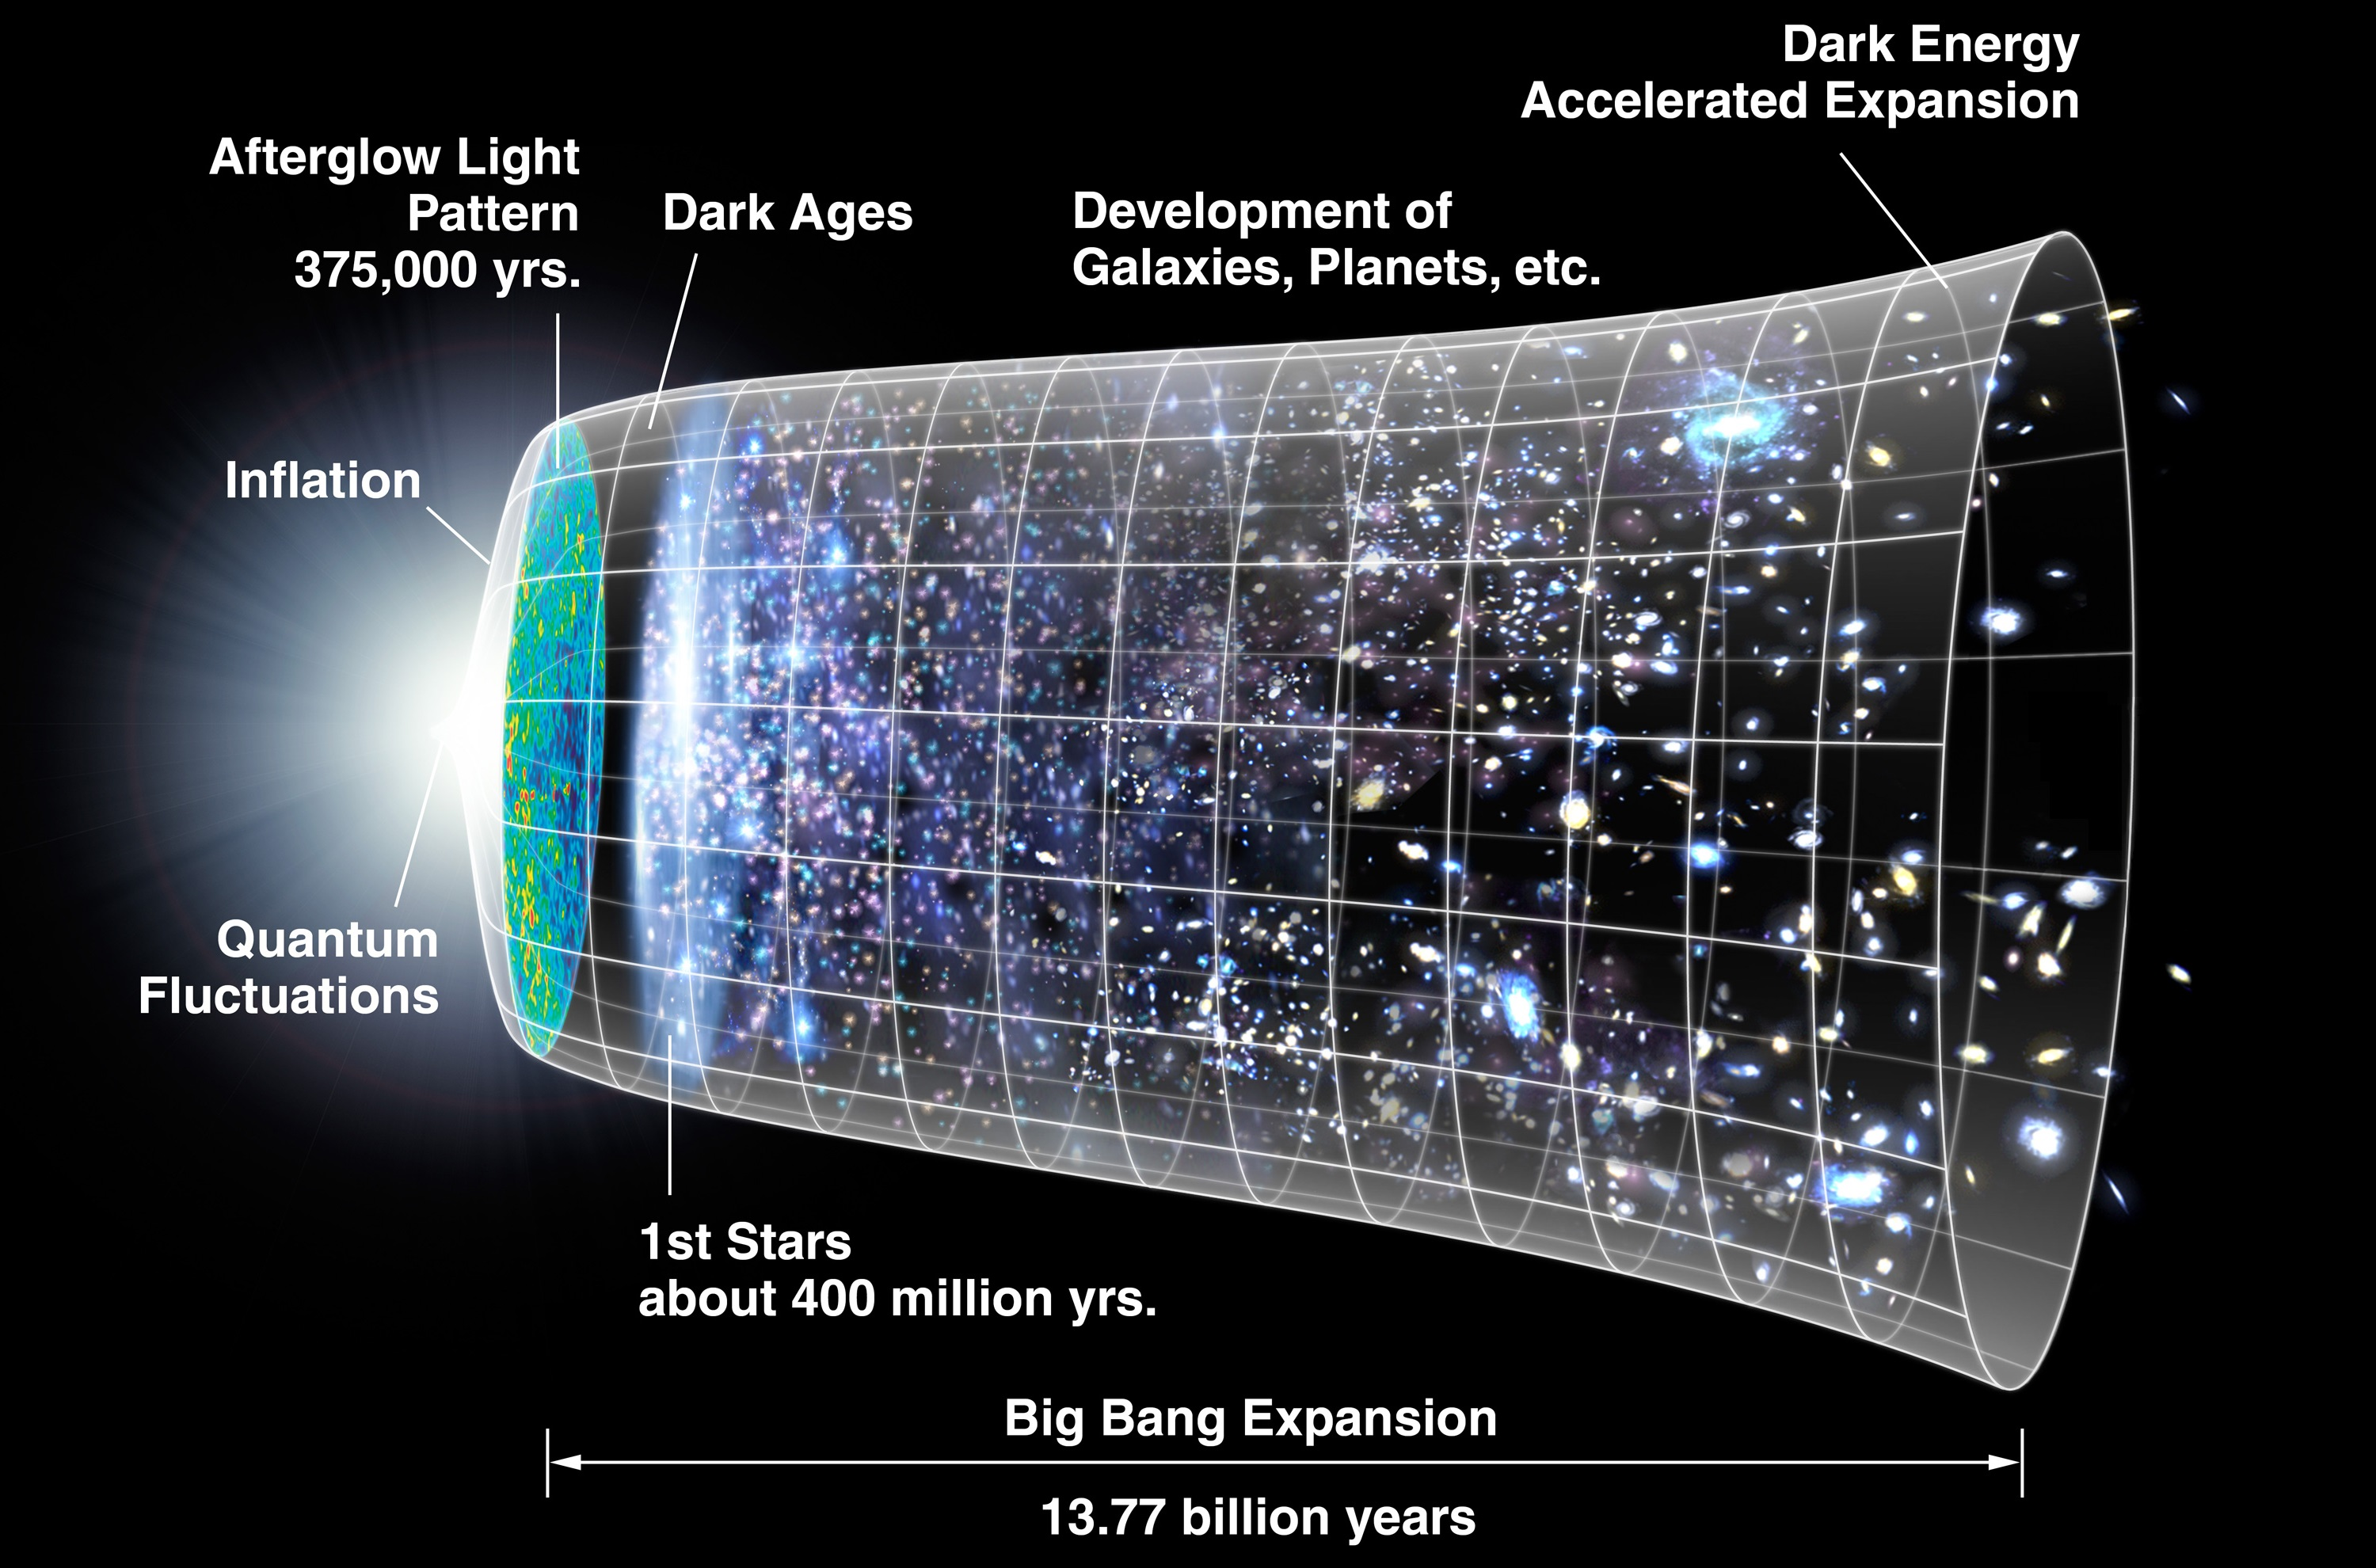
\includegraphics[width=1.0\linewidth]{2_bigbang_expansion.jpeg}
      \vspace{0.2cm}
    \end{column}
    
  \end{columns}

\end{frame}





%-------------------------------------------
% SLIDE 3: RUMORE STRUMENTALE
%-------------------------------------------
\begin{frame}{Caratterizzazione del Rumore Strumentale}

  \begin{columns}[T]
    % --- COLONNA SINISTRA ---
    \begin{column}{0.48\textwidth}
      \metroset{block=transparent}
      \begin{block}{Rumore Bianco}
        \footnotesize
        \begin{itemize}
          \item Spettro di potenza (PSD) piatto.
          \item Campioni indipendenti.
        \end{itemize}
      \end{block}
      
      \centering
      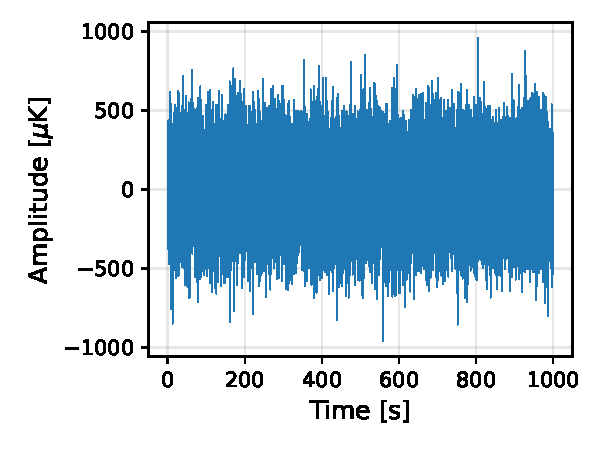
\includegraphics[height=4cm, keepaspectratio]{3_white.pdf}
    \end{column}

    % --- COLONNA DESTRA ---
    \begin{column}{0.48\textwidth}
      \metroset{block=transparent}
      \begin{block}{Rumore $1/f$ (Rosa)}
        \footnotesize
        \begin{itemize}
          \item Dominante alle basse frequenze.
          \item Correlazioni a lungo termine.
        \end{itemize}
      \end{block}

      \centering
      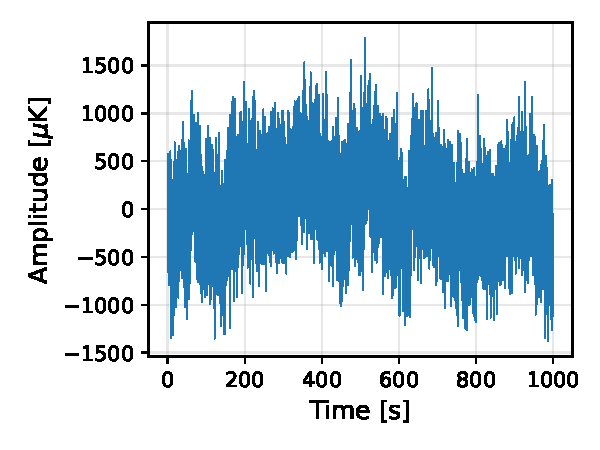
\includegraphics[height=4cm, keepaspectratio]{3_1overf.pdf}
    \end{column}
  \end{columns}

  \vfill
  \vspace{0.1cm}

  \centering
  \small \textbf{Modellizzazione della PSD (Somma dei contributi):} \quad
  $\displaystyle P(f) = \sigma^2 \left[ 1 + \left( \frac{f_{knee}}{f} \right)^\alpha \right]$ 
  
\end{frame}



%-------------------------------------------
% SLIDE 4: IL FRAMEWORK LBS (Corretta - Nota spostata a destra)
%-------------------------------------------
\begin{frame}{Framework LBS (LiteBIRD Simulation)}

  \metroset{block=transparent}
  
  \vspace{0.1cm}
  \begin{block}{Caratteristiche principali}
    \footnotesize
    \begin{itemize}
      \item Libreria Python ufficiale per la simulazione dell'acquisizione dati.
      \item Eseguibile su singolo computer o su cluster HPC. \tikz[remember picture,baseline] \node[anchor=base, xshift=2pt] (n1) {};
      \item Sviluppato per simulazioni End-to-End (E2E).
    \end{itemize}
  \end{block}

  % Nota TikZ spostata ulteriormente a destra (2.5cm) per evitare sovrapposizioni
  \begin{tikzpicture}[remember picture, overlay]
    \node[rectangle, draw=orange!70, fill=orange!5, thick, rounded corners, inner sep=3pt, anchor=west] (note) at ($(n1)+(3cm, 0.0cm)$) {
      \begin{minipage}{3.8cm} % Ridotto leggermente per non uscire a destra della slide
        \fontsize{6pt}{7pt}\selectfont
        \textbf{Setup utilizzato:}\\
        Computer locale (memoria limitata) \\ $\rightarrow$ Implementazione seriale \\$\rightarrow$ Scelte metodologiche
      \end{minipage}
    };
    \draw[->, thick, orange!70] (n1.east) -- (note.west);
  \end{tikzpicture}

  \vspace{-0.5cm}
  \begin{block}{Pipeline E2E}
    \footnotesize
    \begin{enumerate}
      \item Generazione del cielo simulato.
      \item Osservazione del cielo con una strategia di scansione.
      \item Aggiunta del rumore strumentale.
      \item Aggiunta degli effetti sistematici.
      \item Produzione delle mappe finali.
    \end{enumerate}
  \end{block}

  \vspace{-0.1cm}
  
  \begin{center}
    \rule{0.4\textwidth}{0.4pt} \\ \vspace{0.1cm}
    \fontsize{7pt}{8pt}\selectfont
    \textit{LiteBIRD non acquisisce immagini statiche, ma effettua \\ un campionamento continuo del segnale nel tempo.}
  \end{center}

\end{frame}




%-------------------------------------------
% SLIDE 5: STRATEGIA DI SIMULAZIONE
%-------------------------------------------
\begin{frame}{Strategia di Simulazione: Approccio Block-wise}

  \begin{columns}[T]
    \begin{column}{0.75\textwidth}
      \begin{itemize}
        \item \textbf{Sfida:} Enorme volume di dati $\rightarrow$ Il \textbf{TOD} cresce linearmente con il tempo e il numero di detector.
        \item \textbf{Limite:} Elevata occupazione di memoria.
      \end{itemize}
    \end{column}

    \begin{column}{0.25\textwidth}
      \centering
      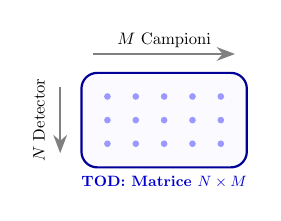
\begin{tikzpicture}[
          scale=0.6, every node/.style={transform shape},
          cell/.style={rectangle, draw=blue!60!black, thick, fill=blue!2, minimum width=3.5cm, minimum height=2cm, rounded corners=2mm},
          axis/.style={-Stealth, thick, gray},
          label/.style={font=\small\bfseries}
      ]
          \node[cell] (Matrix) at (0,0) {};
          \foreach \x in {-1.2, -0.6, 0, 0.6, 1.2} {
              \foreach \y in {-0.5, 0, 0.5} {
                  \fill[blue!40] (\x, \y) circle (2pt);
              }
          }
          \draw[axis] (-2.2, 0.7) -- (-2.2, -0.7) node[midway, left=0.2cm, black, rotate=90, anchor=south] {$N$ Detector};
          \draw[axis] (-1.5, 1.4) -- (1.5, 1.4) node[midway, above, black] {$M$ Campioni};
          \node[label, blue!80!black] at (0, -1.3) {TOD: Matrice $N \times M$};
      \end{tikzpicture}
    \end{column}
  \end{columns}

  \vspace{0.3cm}

  \centering
  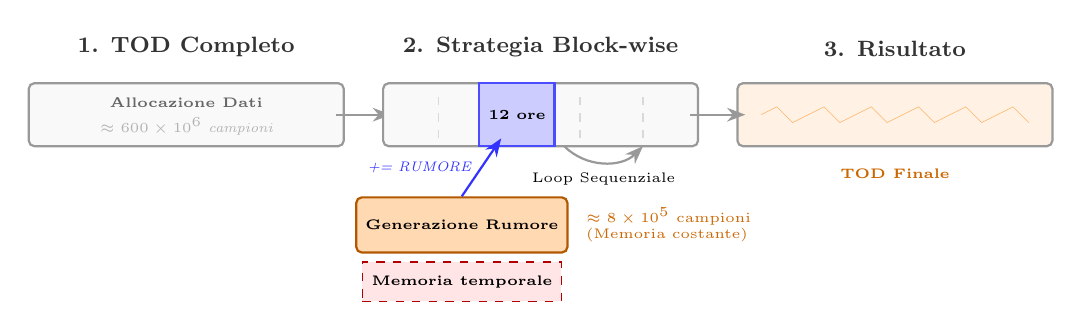
\begin{tikzpicture}[
    node distance=0.5cm,
    tod_base/.style={rectangle, draw=gray!80, thick, minimum width=4cm, minimum height=0.8cm, rounded corners=2pt},
    tod_empty/.style={tod_base, fill=gray!5},
    tod_filled/.style={tod_base, fill=orange!10},
    activeblock/.style={rectangle, draw=blue!70, thick, fill=blue!20, minimum width=0.8cm, minimum height=0.8cm},
    noisebox/.style={rectangle, draw=orange!70!black, thick, fill=orange!30, minimum width=2cm, minimum height=0.7cm, rounded corners=2pt},
    temp_mem/.style={rectangle, draw=red!70!black, dashed, fill=red!10, minimum width=1.5cm, minimum height=0.5cm, font=\tiny\bfseries},
    label/.style={font=\footnotesize\bfseries, text=black!80, align=center},
    arrow/.style={-Stealth, thick, draw=black!40}
]

    % --- STADIO 1 ---
    \node[tod_empty] (T1) at (0, 0) {};
    \node[label, above=0.2cm of T1] {1. TOD Completo};
    \node[font=\tiny\bfseries, color=black!60] at (0,0.15) {Allocazione Dati};
    \node[font=\tiny\itshape, color=gray!60] at (0,-0.15) {$\approx 600 \times 10^6$ campioni};
    \draw[arrow] (1.9, 0) -- (2.6, 0);

    % --- STADIO 2 ---
    \node[tod_empty] (T2) at (4.5, 0) {};
    \node[label, above=0.2cm of T2] {2. Strategia Block-wise};
    
    \foreach \x in {3.2, 3.8, 4.4, 5.0, 5.8} {
        \draw[gray!30, dashed] (\x, -0.3) -- (\x, 0.3);
    }
    
    \node[activeblock] (Current) at (4.2, 0) {\tiny \textbf{12 ore}}; 
    \draw[arrow, bend right=45] (4.8, -0.4) to node[below, font=\fontsize{4}{5}\selectfont] {Loop Sequenziale} (5.8, -0.4);

    % GENERATORE DI RUMORE + MEMORIA TEMPORALE
    \node[noisebox] (Noise) at (3.5, -1.4) {\tiny \textbf{Generazione Rumore}};
    \node[temp_mem, below=0.1cm of Noise] (TempMem) {Memoria temporale};
    \node[right=0.1cm of Noise, font=\tiny, color=orange!80!black, align=left] {$\approx 8 \times 10^5$ campioni\\(Memoria costante)};
    
    \draw[arrow, blue!80] (Noise.north) -- (4.0, -0.3) node[midway, left, font=\tiny\itshape] {+= RUMORE};

    % --- STADIO 3 ---
    \node[tod_filled] (T3) at (9, 0) {};
    \node[label, above=0.2cm of T3] {3. Risultato};
    \draw[very thin, orange!60] (7.3,0) -- (7.5,0.1) -- (7.7,-0.1) -- (7.9,0) -- (8.1,0.1) -- (8.3,-0.1) -- (8.5,0) -- (8.7,0.1) -- (8.9,-0.1) -- (9.1,0) -- (9.3,0.1) -- (9.5,-0.1) -- (9.7,0) -- (9.9,0.1) -- (10.1,-0.1) -- (10.3,0) -- (10.5,0.1) -- (10.7,-0.1);
    \node[font=\tiny\bfseries, color=orange!80!black, below=0.15cm of T3] {TOD Finale};

    \draw[arrow] (6.4, 0) -- (7.1, 0);

\end{tikzpicture}

\end{frame}





%-------------------------------------------
% SLIDE 6: FUNZIONI
%-------------------------------------------
\begin{frame}{Generazione del Rumore: FFT vs Filtri Digitali}

  \begin{columns}[T]
    
    % --- COLONNA SINISTRA: FFT ---
    \begin{column}{0.48\textwidth}
      \metroset{block=transparent}
      \begin{block}{\texttt{add\_lbsNoise} (LBS)}
        \footnotesize
        \textit{Basata su \texttt{add\_noise}} \\
        $\rightarrow$ Trasformata di Fourier (FFT) 
        \begin{itemize}
          \item \textbf{Pro:} 
            \begin{itemize}
                \item Massima flessibilità (PSD arbitrarie).
                \item Facile da parallelizzare.
            \end{itemize}
          \item \textbf{Contro:} 
            \begin{itemize}
                \item Elevato uso di memoria ($\propto \mathcal{O}(M)$).
                \item Discontinuità ai bordi dei blocchi.
            \end{itemize}
        \end{itemize}
      \end{block}

      \vspace{0.2cm}
      \centering
      \scalebox{0.7}{
        $\displaystyle P(f) = \frac{\sigma^{2}}{f_{\text{samp}}} \left[ \frac{f^\alpha + f_{\text{knee}}^\alpha}{f^\alpha + f_{\text{min}}^\alpha} \right]$
      }
    \end{column}

    % --- COLONNA DESTRA: FILTRI ---
    \begin{column}{0.48\textwidth}
      \metroset{block=transparent}
      \begin{block}{\texttt{add\_OofaNoise} (\texttt{ducc0})}
        \footnotesize
        \textit{Basata su \texttt{OofaNoise}} \\
        $\rightarrow$ Filtri digitali ricorsivi
        \begin{itemize}
          \item \textbf{Pro:} 
            \begin{itemize}
                \item \textbf{Continuità temporale} tra i blocchi.
                \item Memoria minima e costante ($\sim 200 \ Byte$).
            \end{itemize}
          \item \textbf{Contro:} 
            \begin{itemize}
                \item Rigidità spettrale.
                \item Più difficile da parallelizzare.
            \end{itemize}
        \end{itemize}
      \end{block}

      \vspace{0.2cm}
      \centering
      \scalebox{0.7}{
        $\displaystyle P(f) = \frac{\sigma^{2}}{f_{\text{samp}}} \left[ \frac{f^{2} + f_{\text{knee}}^{2}}{f^{2} + f_{\text{min}}^{2}} \right]^{\alpha/2}$
      }
    \end{column}

  \end{columns}

  \vfill
  \centering
  \scriptsize\textit{Nota: Entrambi i modelli sono approssimazioni analitiche della complessità reale dei detector.}

\end{frame}






%-------------------------------------------
% SLIDE 7: PIPELINE DI SIMULAZIONE
%-------------------------------------------
\begin{frame}{Pipeline di Simulazione}

  % --- PARTE ALTA: WORKFLOW ---
  \metroset{block=transparent}
  \begin{block}{Workflow di Validazione}
    \small
    \begin{enumerate}
      \item Definizione strategia scansione.
      \item Configurazione detector.
      \item Generazione dati.
      \item Analisi: dominio tempo, dominio frequenza, mappe e dominio armoniche sferiche.
    \end{enumerate}
  \end{block}

  \vspace{0.4cm}

  % --- PARTE BASSA: TABELLA ---
  \centering
  \small
  \rowcolors{2}{gray!5}{white}
  \begin{tabular}{p{6cm}c}
    \toprule
    \textbf{Parametri Detector} & \textbf{Custom} \\
    \midrule
    Frequenza di Campionamento [$f_{samp}$] & $20.0$ Hz \\
    Sensibilità (NET) & $50.0\,\mu\text{K}\sqrt{\mathrm{s}}$ \\
    Frequenza di Ginocchio ($f_{knee}$) & $500.0$ mHz \quad 
    \tikz[baseline=(char.base)]{\node[red, font=\bfseries\tiny, draw=red, rounded corners=2pt, inner sep=2pt] (char) {ESAGERATO}; \draw[stealth-, red, thick] (char.west) -- ++(-0.4,0);} \\
    Frequenza Minima ($f_{min}$) & $10^{-5}$ Hz \\
    Indice Spettrale $\alpha$ & $1.0$ \\
    \bottomrule
  \end{tabular}

  \vspace{0.3cm}
  \scriptsize\textit{Nota: I parametri sono scelti per massimizzare la visibilità del rumore $1/f$.}

\end{frame}






%-------------------------------------------
% SLIDE 8: DOMINIO TEMPORALE
%-------------------------------------------
\begin{frame}{Analisi nel Dominio del Tempo (TOD)}

  \begin{columns}[c] 
    
    % --- COLONNA SINISTRA: GRAFICI (Larghezza corretta) ---
    \begin{column}{0.62\textwidth}
      \centering
      
      % Primo Grafico: FFT
      \begin{figure}
        \centering
        \begin{subfigure}{\textwidth}
          \centering
          \scriptsize \textbf{add\_lbsNoise} (FFT)\\
          \vspace{0.05cm}
          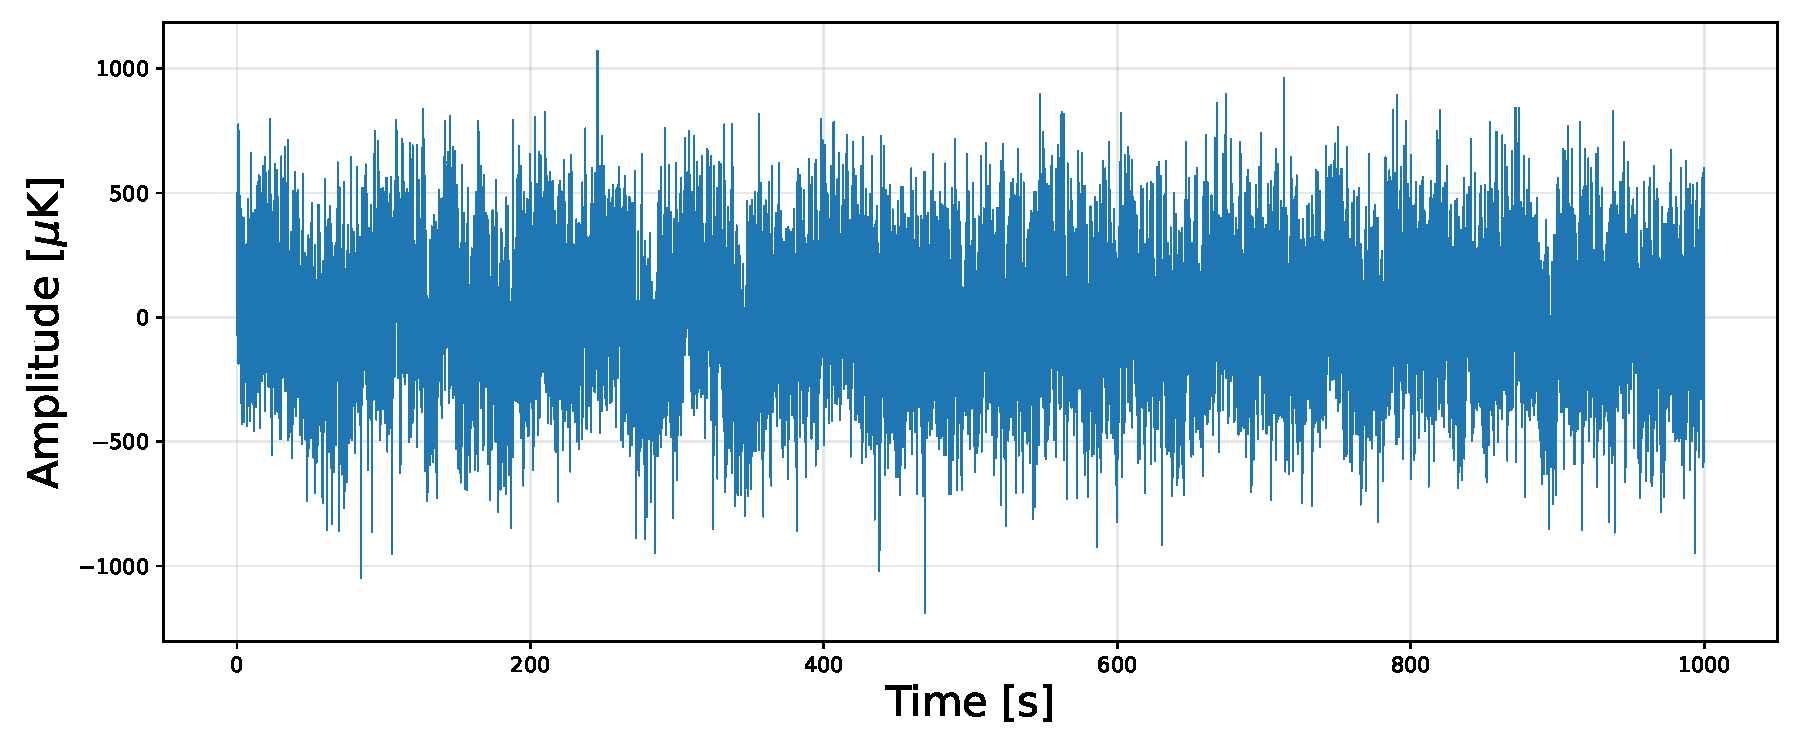
\includegraphics[width=0.92\linewidth]{tod_mock_lbs.pdf}
        \end{subfigure}

        \vspace{0.2cm} % Distanza bilanciata tra i due grafici
        
        % Secondo Grafico: OOFA
        \begin{subfigure}{\textwidth}
          \centering
          \scriptsize \textbf{add\_OofaNoise} (Filtri)\\
          \vspace{0.05cm}
          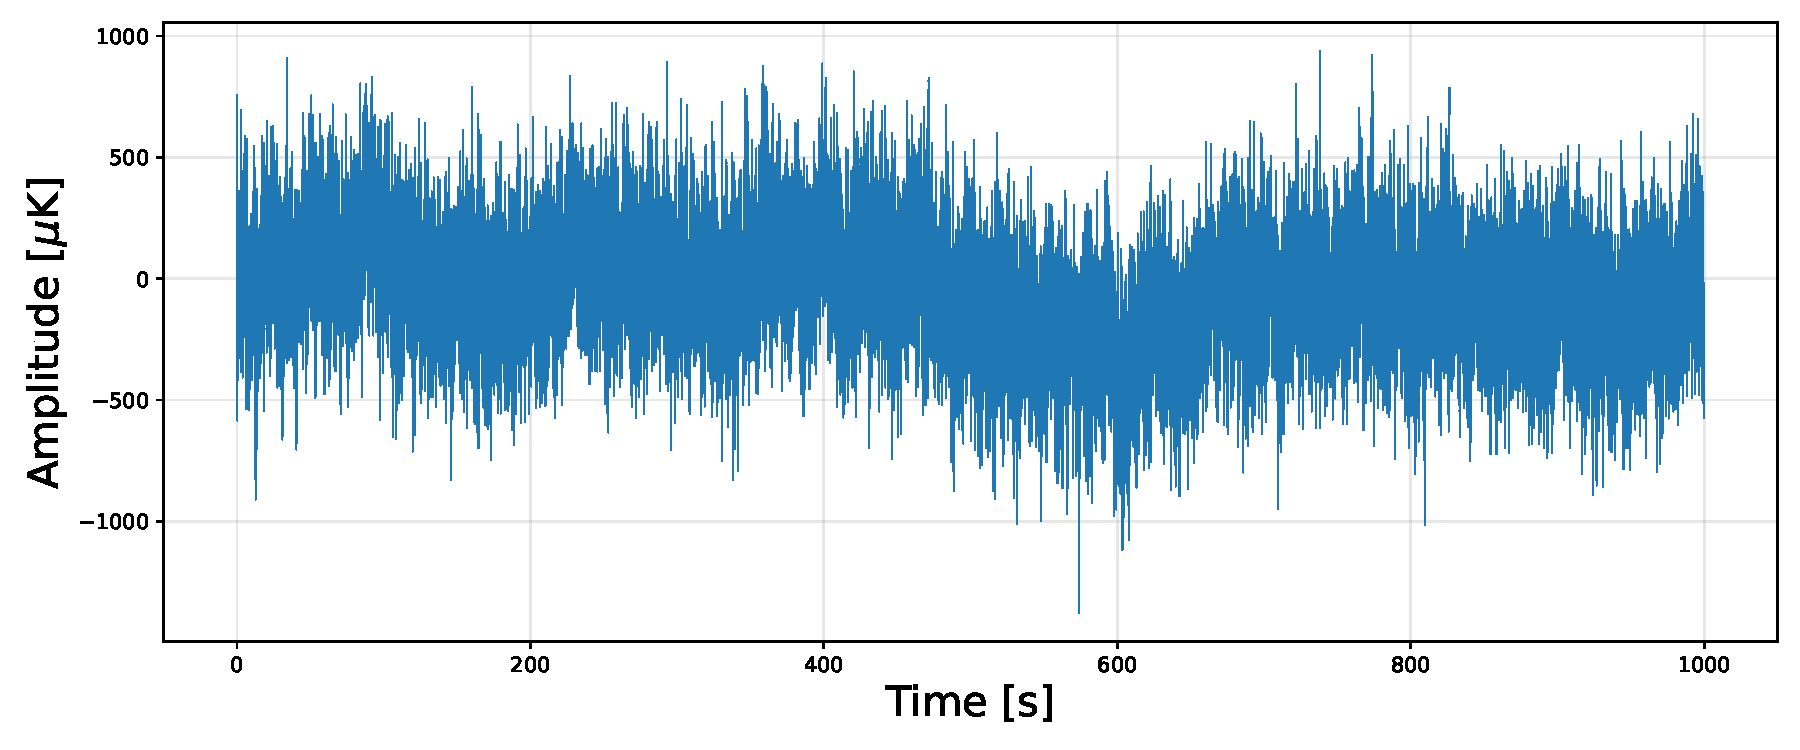
\includegraphics[width=0.92\linewidth]{tod_mock_oofa.pdf}
        \end{subfigure}
      \end{figure}
    \end{column}

    % --- COLONNA DESTRA: PUNTI CHIAVE ---
    \begin{column}{0.38\textwidth} % Ridotta per non sforare il 100%
      \metroset{block=transparent}
      
      \begin{itemize}
        \item \footnotesize \textbf{Configurazione:} Custom detector, 1000\,s (blocchi 100\,s). 
        \item \footnotesize \textbf{Componenti:} 
          \begin{itemize}
            \item \scriptsize \textit{Bianco:} oscillazioni rapide. 
            \item \scriptsize \textit{$1/f$:} drift lenti. 
          \end{itemize}
      \end{itemize}

      \vspace{0.2cm}

    \begin{alertblock}{Continuità Temporale}
        \fontsize{6pt}{7pt}\selectfont
        \begin{itemize}
          \item FFT: Correlazioni spezzate ogni 100\,s $\rightarrow$ segnale non si allontana dallo zero.
          \item Filtri: Transizione fluida tra blocchi $\rightarrow$ segnale libero di evolvere.
        \end{itemize}
      \end{alertblock}
      
    \end{column}
  \end{columns}


\end{frame}





%-------------------------------------------
% SLIDE 9: DOMINIO DELLE FREQUENZE
%-------------------------------------------
\begin{frame}{Caratterizzazione nel Dominio delle Frequenze (PSD)}

  \begin{columns}[c]
    
    % --- COLONNA SINISTRA: METODOLOGIA E ANALISI ---
    \begin{column}{0.38\textwidth}
      \metroset{block=transparent}
      
      \begin{block}{Stima Spettrale: Metodo di Welch}
        \scriptsize
        $\rightarrow$ Consistente rispetto al periodogramma classico.
        \begin{itemize}
          \item \textbf{Segmentazione} e overlap (50\%).
          \item \textbf{Windowing} $\rightarrow$ Riduzione leakage.
          \item \textbf{Media} $\rightarrow$ Riduzione varianza.
          \item \textbf{Risoluzione:} $\approx 5$\,mHz.
        \end{itemize}
      \end{block}

      \vspace{0.1cm}

      \begin{itemize}
        \item \footnotesize \textbf{Risultati:}
          \begin{itemize}
            \item \scriptsize Accordo con modello analitico.
            \item \scriptsize Plateau bianco e risalita $1/f$.
          \end{itemize}
        \end{itemize}

    \vspace{0.2cm}

  % --- AGGIUNTA ALERTBLOCK PER IL PROF ---
  \begin{alertblock}{Discrepanza per metodo FFT}
    \fontsize{6pt}{7pt}\selectfont
    Perdita di potenza alle basse frequenze rispetto allo spettro teorico. \\ 
    $\rightarrow$ Correlato alla lunghezza del chunk.
  \end{alertblock}
    
    \end{column}

    % --- COLONNA DESTRA: GRAFICI PSD ---
    \begin{column}{0.62\textwidth}
      \centering
      \begin{figure}
        \begin{subfigure}{\textwidth}
          \centering
          \scriptsize \textbf{add\_lbsNoise} (FFT)\\
          \vspace{0.05cm}
          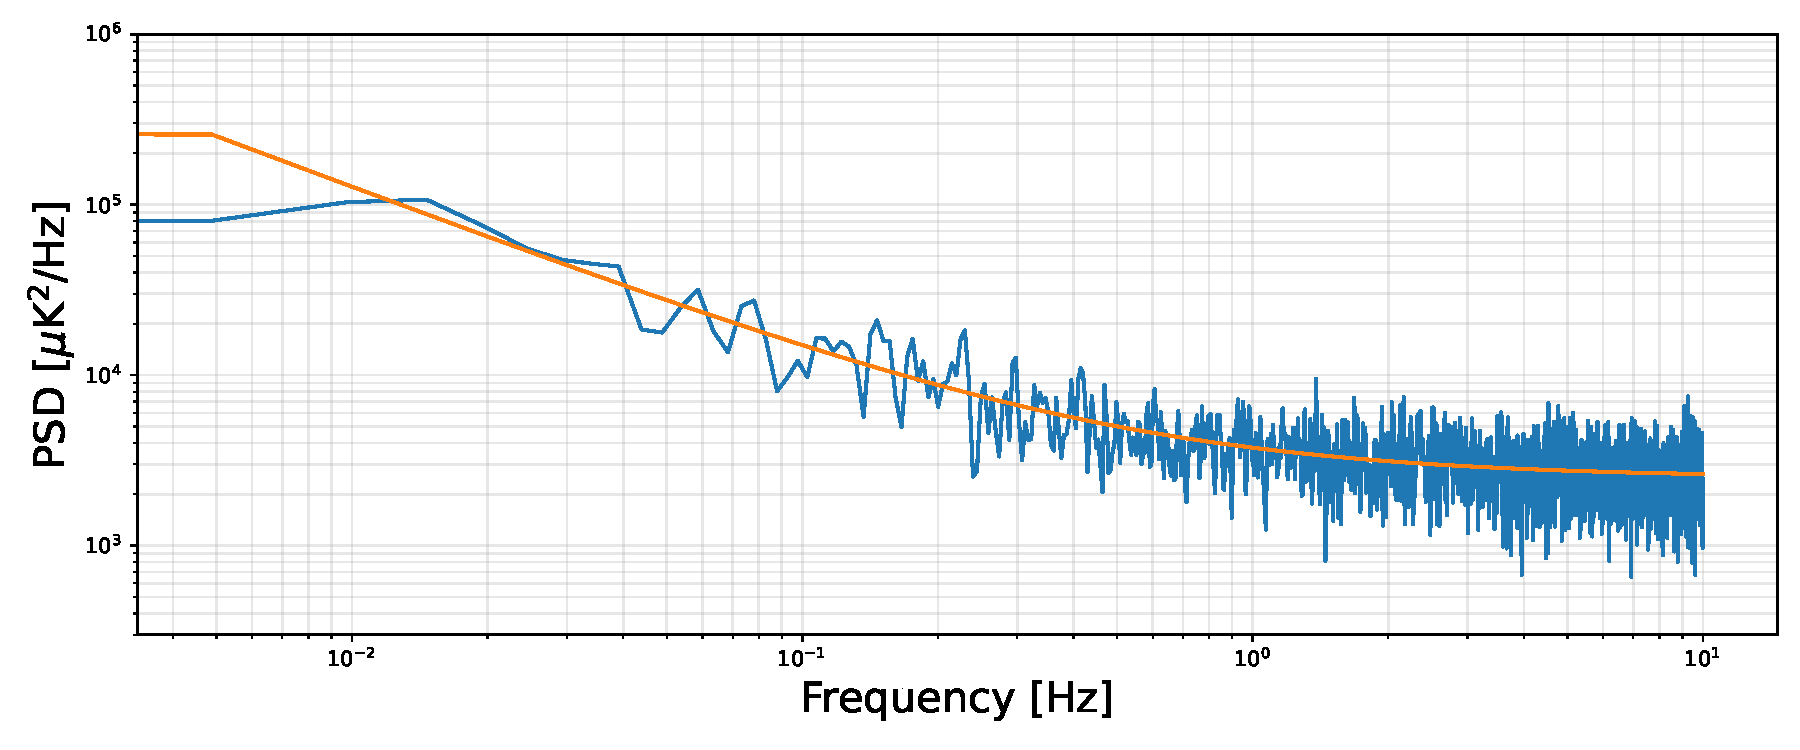
\includegraphics[width=0.92\linewidth]{psd_mock_lbs.pdf}
        \end{subfigure}

        \vspace{0.1cm}

        \begin{subfigure}{\textwidth}
          \centering
          \scriptsize \textbf{add\_OofaNoise} (Filtri)\\
          \vspace{0.05cm}
          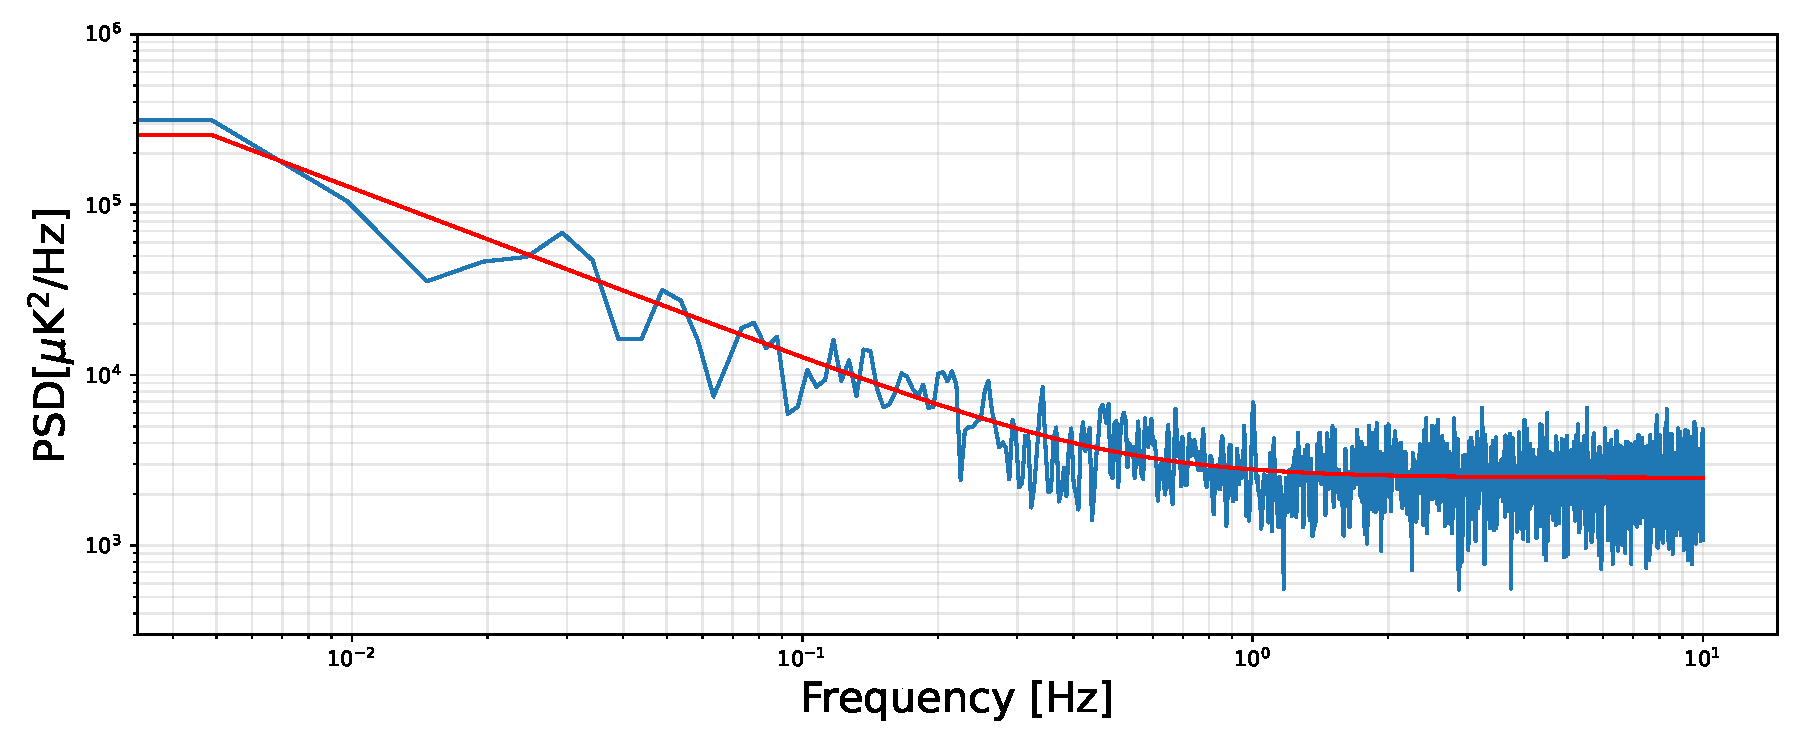
\includegraphics[width=0.92\linewidth]{psd_mock_oofa.pdf}
        \end{subfigure}
      \end{figure}
    \end{column}

  \end{columns}

\end{frame}






%-------------------------------------------
% SLIDE 10: MAP-MAKING E BINNING
%-------------------------------------------
\begin{frame}{Map-making e Algoritmo di Binning}

  % --- PARTE ALTA: CONFIGURAZIONE ---
  \metroset{block=transparent}
  \begin{block}{Simulazione Missione}
    \footnotesize
    1 anno di osservazione ($\approx 600 \times 10^6$ campioni) $\rightarrow$ Blocchi da 12h.
  \end{block}

  \vspace{0.3cm}

  % --- PARTE CENTRALE: LE MAPPE ---
  \begin{columns}[T]
    \begin{column}{0.48\textwidth}
      \centering
      \small \textbf{Hit-map} \\
      \scriptsize Copertura del cielo: conteggio campioni per pixel. \\
      \textit{Dipende solo dalla strategia di scansione.}
    \end{column}
    \begin{column}{0.48\textwidth}
      \centering
      \small \textbf{Mappa di solo rumore} \\
      \scriptsize Proiezione dei campioni TOD. \\
      \textit{Assenza di segnale astrofisico.}
    \end{column}
  \end{columns}

  \vspace{0.4cm}

  % --- PARTE BASSA: ALGORITMO E FORMULA ---
  \begin{exampleblock}{Algoritmo di Binning}
    \centering
    \vspace{0.1cm}
    $\displaystyle m(p) = \frac{1}{N_p} \sum_{i \in p} d_i$
    \vspace{0.1cm}
  \end{exampleblock}

  \vspace{0.4cm}

  \centering
  \footnotesize 
  $\rightarrow$ \textbf{Destriping:} Metodo più semplice per la rimozione del rumore $1/f$. \\
  \vspace{0.1cm}
  \scriptsize \textit{Non applicato per evidenziare le striature $1/f$.}

\end{frame}







%-------------------------------------------
% SLIDE 11: MAPPE DI RUMORE 
%-------------------------------------------
\begin{frame}{Mappe e Pattern di Rumore}

  % --- PROIEZIONE MOLLWEIDE (ALTO A DX) ---
  \begin{tikzpicture}[remember picture, overlay]
    \node[anchor=north east, xshift=-0cm, yshift=-1.0cm] at (current page.north east) {
      \begin{tabular}{c}
        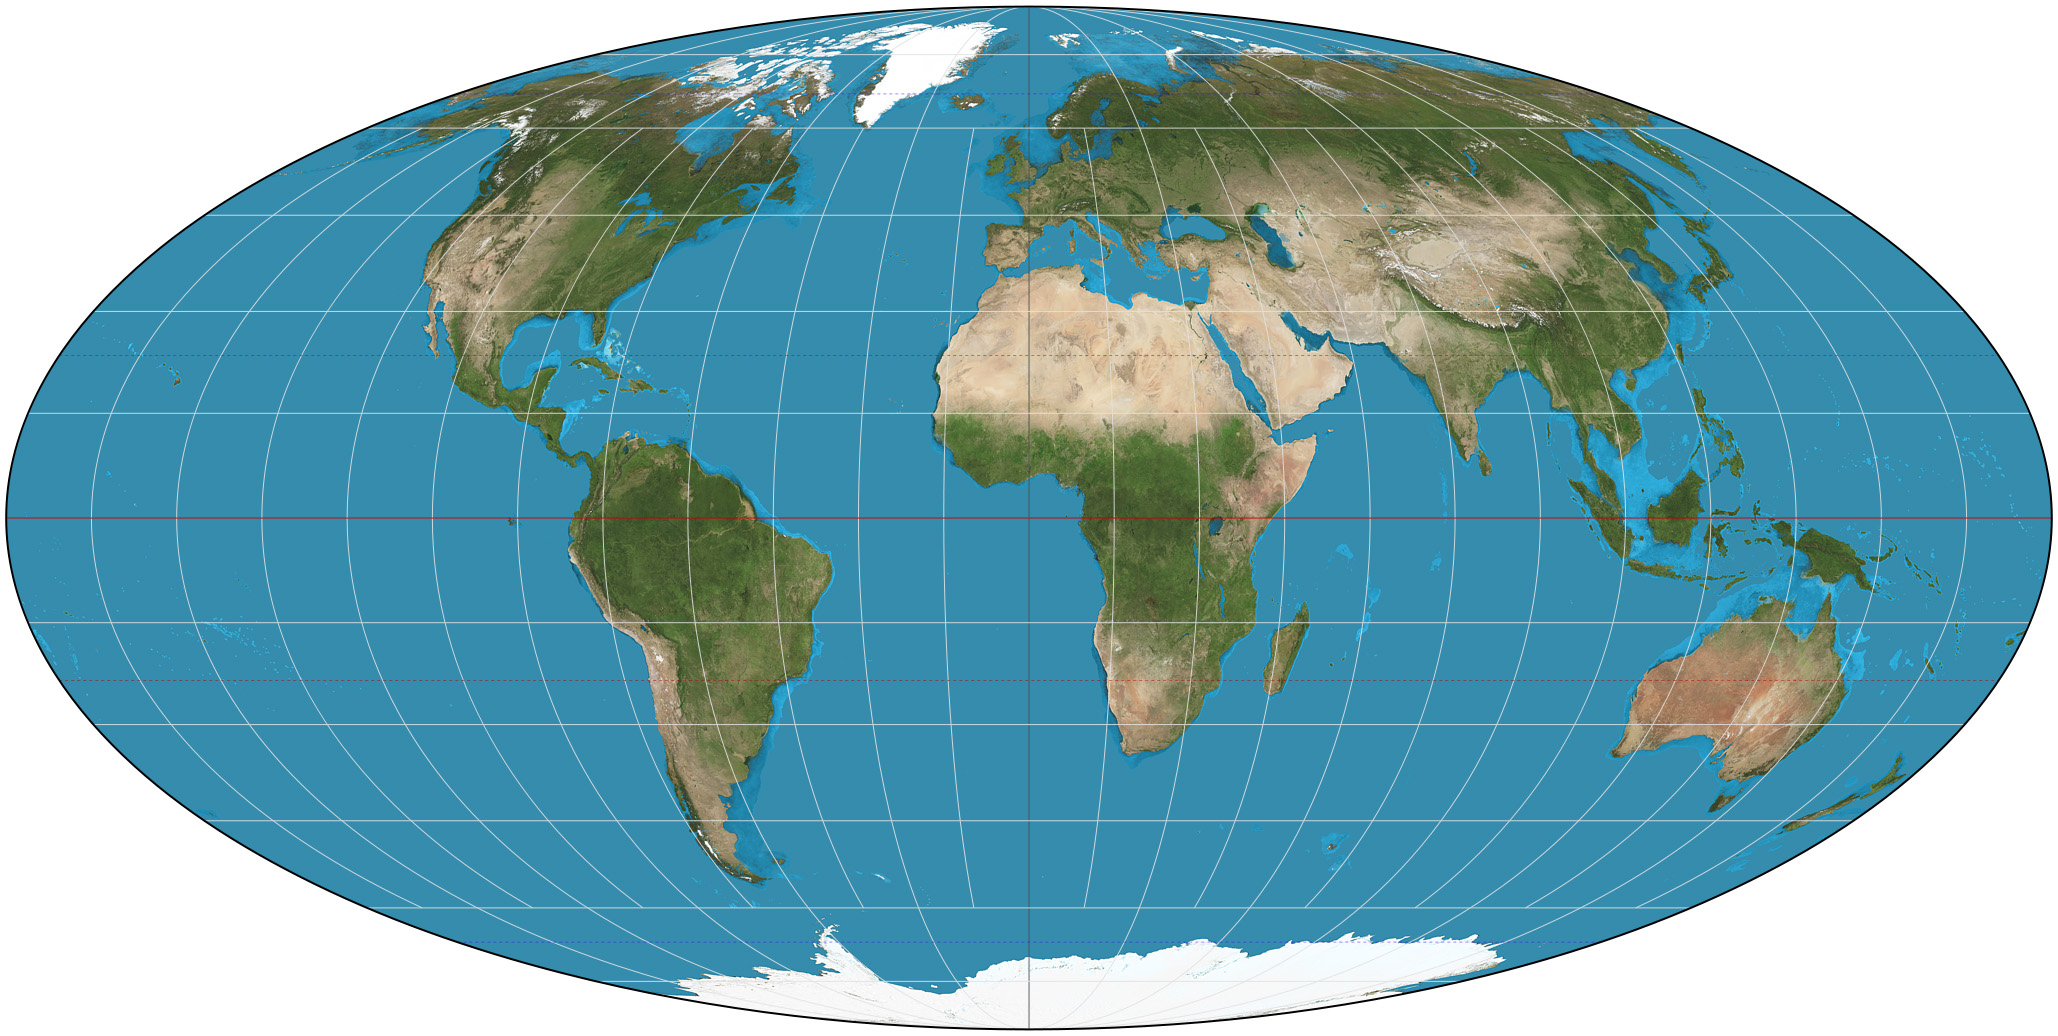
\includegraphics[width=1.8cm]{Mollweide_projection_SW.jpeg} \\
      \end{tabular}
    };
  \end{tikzpicture}

  % --- MAPPE DI RUMORE (AL CENTRO) ---
  % Ridotto width delle immagini al 90% per recuperare spazio verticale
  \begin{columns}[t]
    \begin{column}{0.48\textwidth}
      \centering
      {\color{mDarkTeal} \scriptsize \textbf{add\_lbsNoise} (FFT)}\\
      \vspace{0.05cm}
      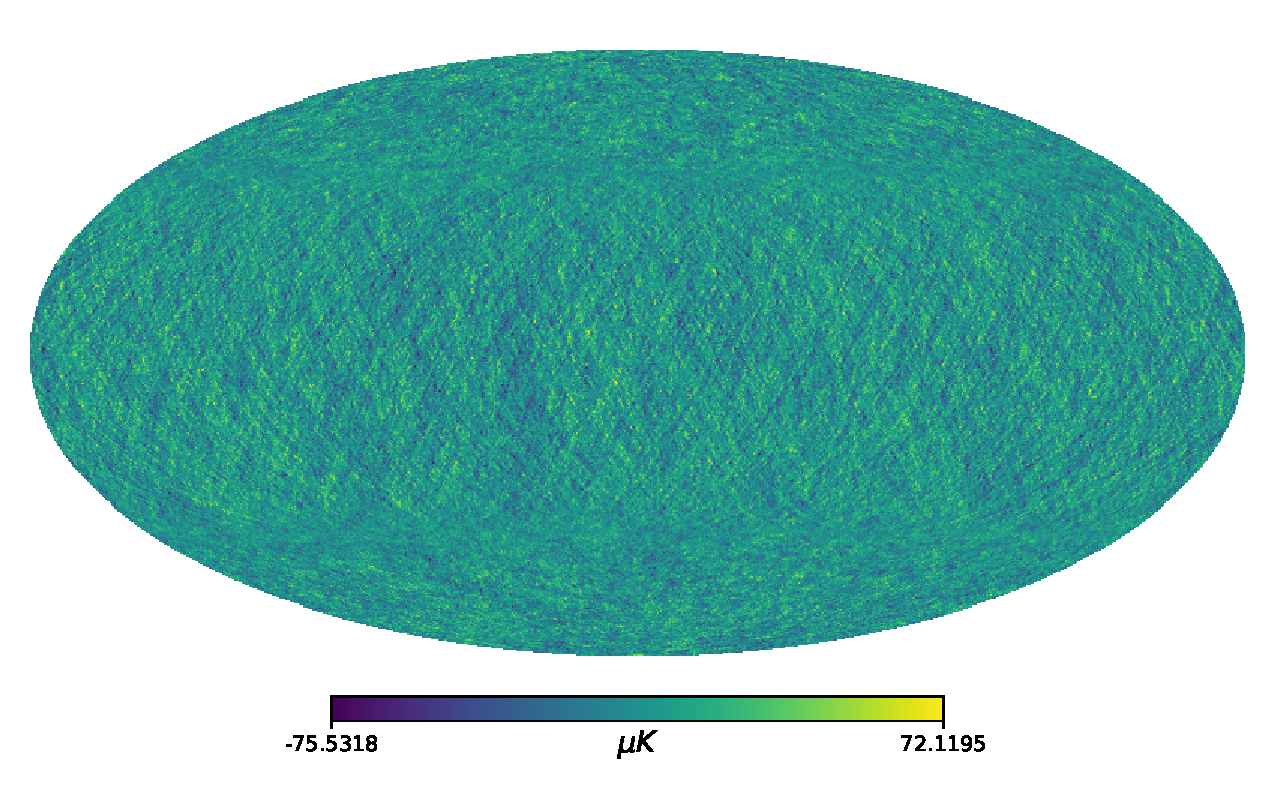
\includegraphics[width=0.9\linewidth]{noise_map_lbs.pdf}
    \end{column}
    \hspace{0.05cm} 
    \begin{column}{0.48\textwidth}
      \centering
      {\color{mDarkTeal} \scriptsize \textbf{add\_OofaNoise} (Filtri)}\\
      \vspace{0.05cm}
      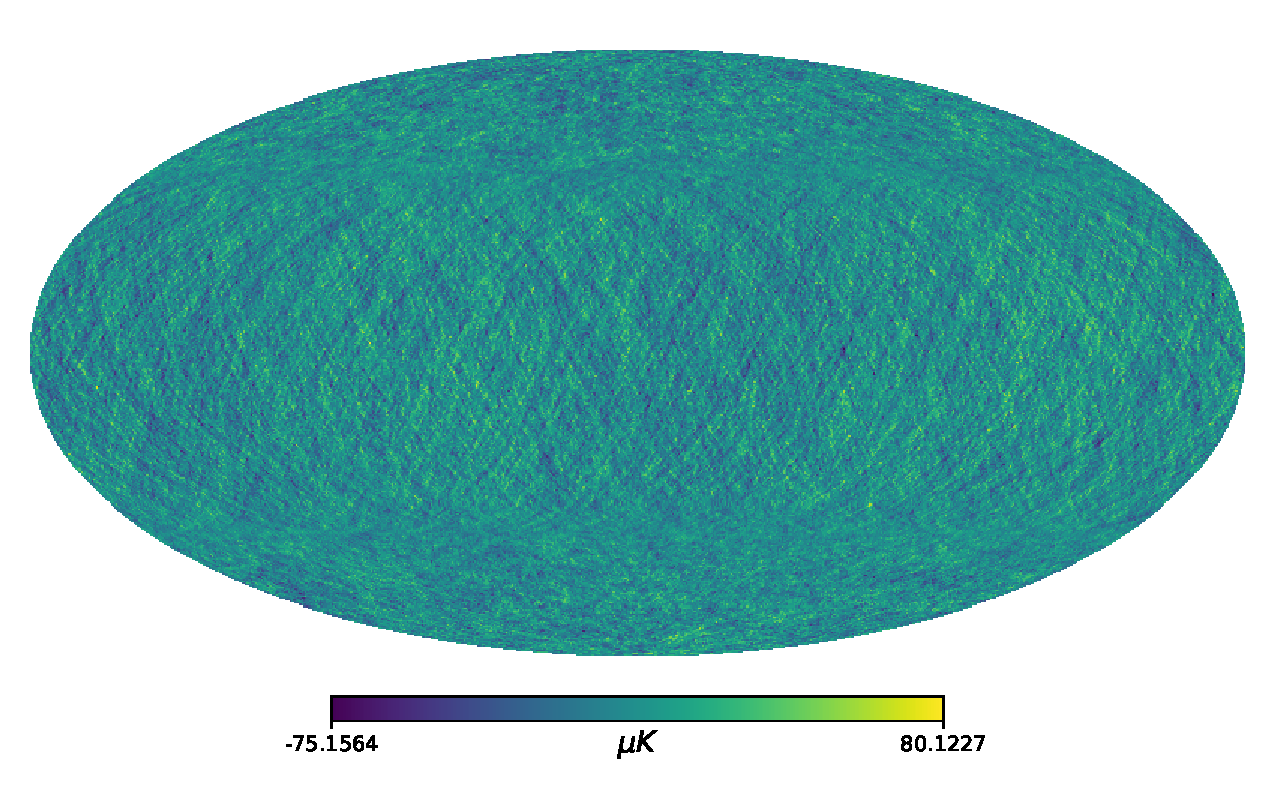
\includegraphics[width=0.9\linewidth]{noise_map_oofa.pdf}
    \end{column}
  \end{columns}

  \vspace{0.2cm}
  \hrule 
  \vspace{0.1cm}

  % --- ANALISI IN BASSO ---
  \metroset{block=transparent}
  \begin{block}{Analisi Morfologica}
    \fontsize{8pt}{9pt}\selectfont
    \begin{itemize}
      \item \textbf{Grana fine:} Fluttuazioni isotropiche (rumore bianco).
      \item \textbf{Striature:} Correlazioni $1/f$ a larga scala.
    \end{itemize}
  \end{block}

  \vfill 
  
  \centering
  \fontsize{7pt}{8pt}\selectfont
  Ho validato i modelli anche nel dominio delle armoniche sferiche tramite l'analisi dello \textbf{spettro di potenza angolare} ($C_\ell$).

\end{frame}



%-------------------------------------------
% SLIDE 12: CONCLUSIONI E PROSPETTIVE FUTURE
%-------------------------------------------
\begin{frame}{Conclusioni e Prospettive Future}

  \metroset{block=transparent}

  % --- PARTE SUPERIORE: RISULTATI ---
  \begin{block}{Risultati}
    \footnotesize
    \begin{itemize}
      \item \textbf{Efficienza strategia \textit{block-wise}:} Simulazioni di un intero anno di missione.
      \item \textbf{Confronto tra i modelli di rumore:}
        \begin{itemize}
          \scriptsize
          \item Continuità temporale del segnale tra i blocchi.
          \item Riduzione dei tempi di calcolo e consumo costante di memoria.
          \item Preservazione della validità statistica (PSD e $C_\ell$).
        \end{itemize}
    \end{itemize}
  \end{block}

  \vspace{0.4cm}

  % --- PARTE CENTRALE: SVILUPPI ---
  \begin{block}{Sviluppi Futuri}
    \footnotesize
    \begin{itemize}
      \item Estensione al caso \textbf{multi-detector}.
      \item Integrazione in una \textbf{pipeline End-to-End (E2E)}.
    \end{itemize}
  \end{block}

\end{frame}
\appendix







%-------------------------------------------
% SLIDE: Grazie
%-------------------------------------------
\begin{frame}[noframenumbering]
\begin{center}
\vspace{2cm}
{\Large\textbf{Grazie per l'attenzione}}

\vspace{1.5cm}
\end{center}
\end{frame}


















%-------------------------------------------
% SLIDE: Backup Slides
%-------------------------------------------
\setbeamercolor{frametitle}{bg=ottanio,fg=white}
\setbeamercolor{palette primary}{bg=ottanio,fg=white}



%-------------------------------------------
% SLIDE A: HIT-MAP E ATTENUAZIONE
%-------------------------------------------
\begin{frame}{Backup: Hit-Map e Attenuazione}
  
  \begin{columns}[T]
    % Colonna Sinistra
    \begin{column}{0.48\textwidth}
      \centering
      \small \textbf{Hit-map} \\
      \vspace{0.1cm}
      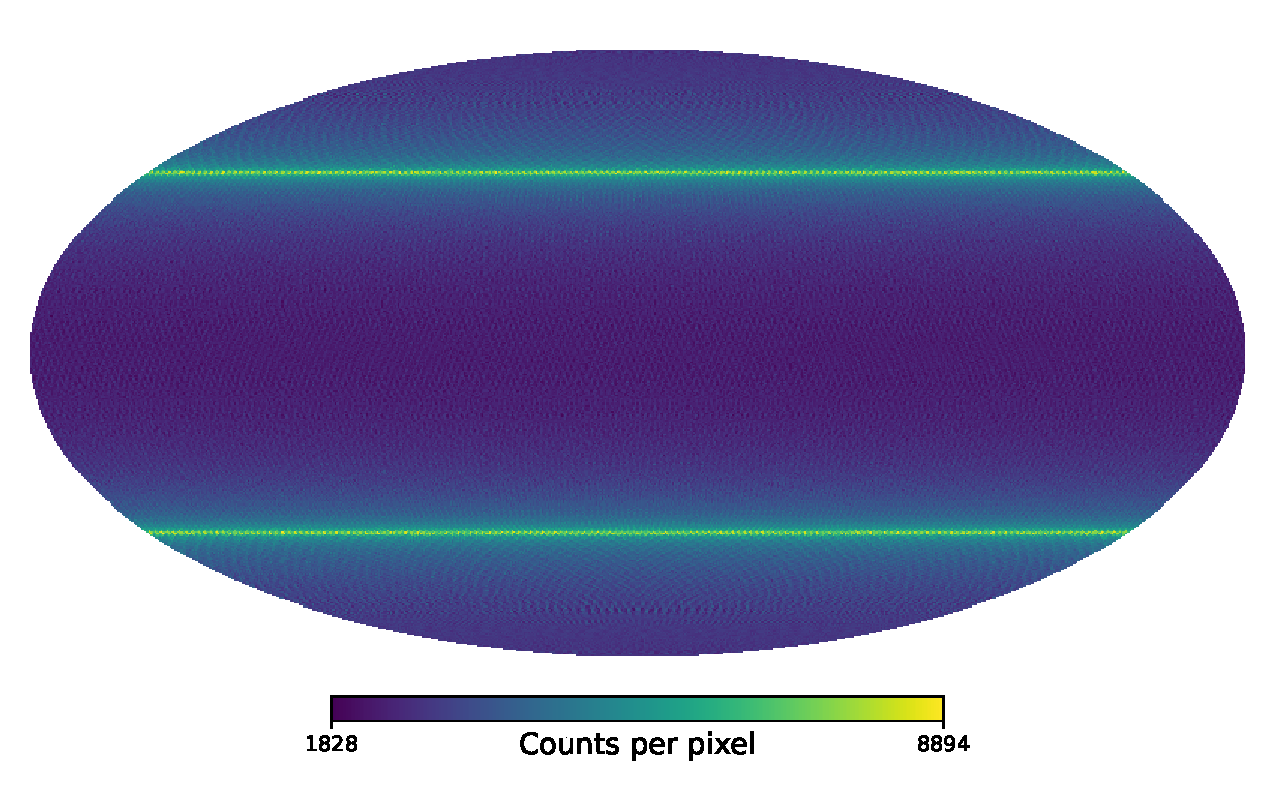
\includegraphics[width=0.9\linewidth]{hit_map.pdf}
      
      \vspace{0.4cm}
      
      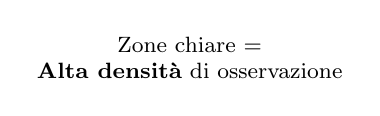
\begin{tikzpicture}[remember picture]
        \node (dens) [align=center, font=\footnotesize] {Zone chiare = \\ \textbf{Alta densità} di osservazione};
      \end{tikzpicture}
    \end{column}

    % Colonna Destra
    \begin{column}{0.48\textwidth}
      \centering
      \small \textbf{Mappa di Rumore} \\
      \vspace{0.1cm}
      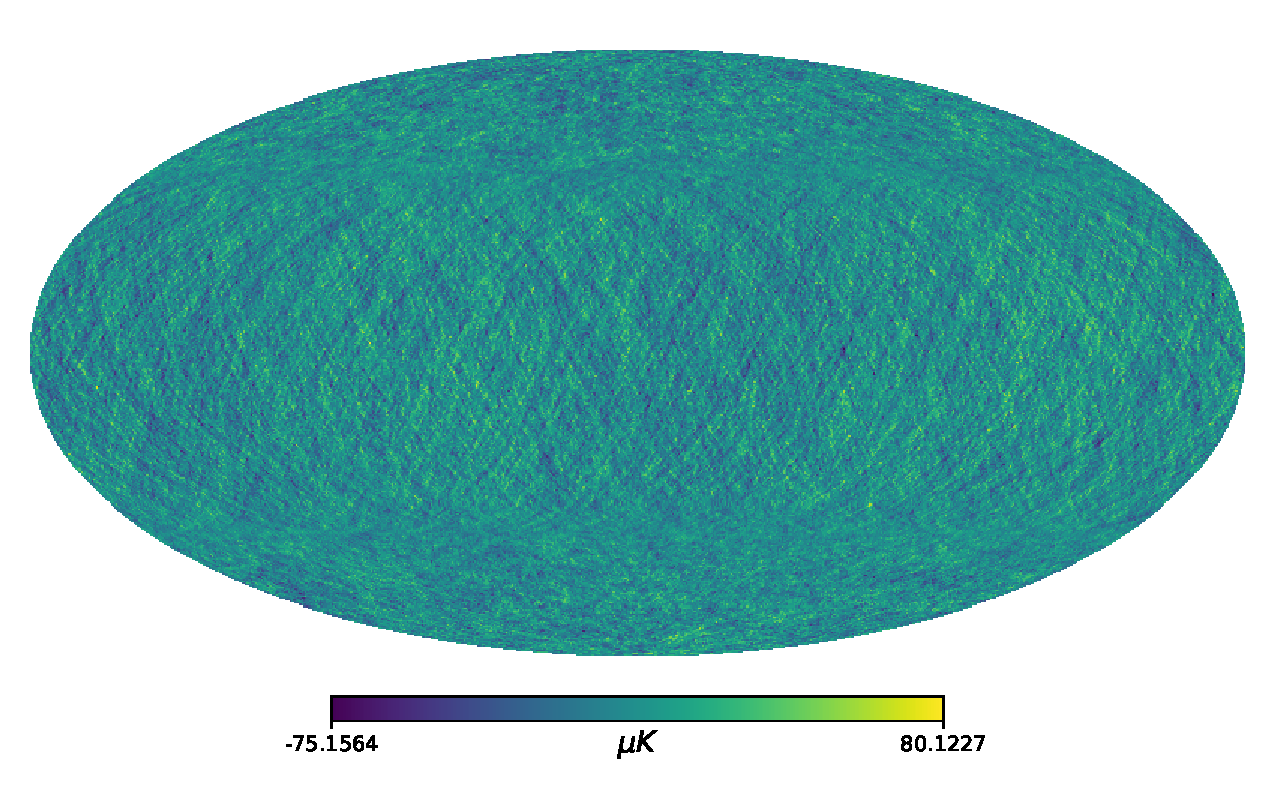
\includegraphics[width=0.9\linewidth]{noise_map_oofa.pdf}
      
      \vspace{0.4cm}
      
      
\begin{tikzpicture}[remember picture]
        \node (canc) [align=center, font=\footnotesize] {
            \textbf{Cancellazione statistica} dei drift \\ 
            Attenuazione delle striature $1/f$
        };
      \end{tikzpicture}
    \end{column}
  \end{columns}

  \vspace{0.4cm}

  % Blocco Finale centrato senza freccia in entrata
  \centering
  \begin{tikzpicture}[remember picture, arrow/.style={-Stealth, thick, mDarkTeal}]
    \node (filt) [align=center, font=\footnotesize] {
        La \textbf{ridondanza} della scansione agisce come \\ \textbf{primo filtro naturale}
    };

    % Unica freccia orizzontale tra i nodi superiori
    \draw[arrow, overlay] (dens.east) -- (canc.west);
  \end{tikzpicture}

\end{frame}




%-------------------------------------------
% SLIDE B: RISOLUZIONE (HEALPix)
%-------------------------------------------
\begin{frame}{Backup: Risoluzione Mappe}

  \begin{columns}[T]
    % --- COLONNA SINISTRA: TEORIA ---
    \begin{column}{0.48\textwidth}
      \metroset{block=transparent}
      \begin{block}{Caratteristiche di HEALPix}
        \fontsize{7pt}{8pt}\selectfont
        \textit{Hierarchical Equal Area isoLatitude Pixelization}
        \begin{itemize}
          \item \textbf{Area Equivalente:} Ogni pixel copre lo stesso angolo solido.
          \item \textbf{Struttura Gerarchica:} Suddivisione ricorsiva dei 12 pixel di base.
          \item \textbf{Iso-latitudine:} Centri dei pixel su anelli di latitudine costante.
        \end{itemize}
      \end{block}

      \centering
      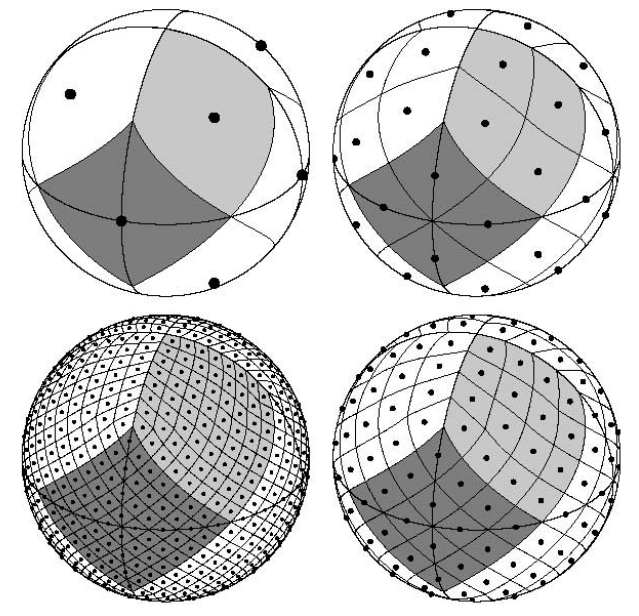
\includegraphics[width=0.5\linewidth]{2_healpix.png}
    \end{column}

    % --- COLONNA DESTRA: TUA CONFIGURAZIONE ---
    \begin{column}{0.48\textwidth}
      \metroset{block=transparent}
      \begin{block}{Risoluzione della Simulazione}
        \footnotesize
        Parametro di risoluzione scelto:
        \centering
        \textbf{$N_{\text{side}} = 2^7 = 128$}
      \end{block}

      \vspace{0.1cm}
      \rowcolors{2}{gray!5}{white}
      \scriptsize
      \begin{tabular}{ll}
        \toprule
        \textbf{Parametro} & \textbf{Valore} \\
        \midrule
        Numero totale pixel ($12 N_{\text{side}}^2$) & $196.608$ \\
        Dimensione pixel ($\theta_{\text{pix}}$) & $\approx 27.5'$ \\
        Multipolo massimo ($\ell_{\text{max}} = 3N_{\text{side}}-1$) & $383$ \\
        \bottomrule
      \end{tabular}

      \vspace{0.3cm}
      \centering
      \scriptsize \textit{$\rightarrow$ con un $N_{\text{side}}$ più alto dominerebbe il rumore bianco sul singolo pixel.}
      
    \end{column}
  \end{columns}

\end{frame}



%-------------------------------------------
% SLIDE C: LO SPETTRO DI POTENZA ANGOLARE
%-------------------------------------------
\begin{frame}{Backup: Spettro di Potenza Angolare ($C_\ell$)}
  \begin{columns}[T]
    % --- COLONNA SINISTRA: EQUAZIONI ---
    \begin{column}{0.5\textwidth}
      \metroset{block=transparent}
      \begin{block}{Analisi Armonica sulla Sfera}
        \footnotesize
        Espansione della mappa in armoniche sferiche $Y_{\ell m}$:
        \[ \Delta T(\theta, \phi) = \sum_{\ell=0}^{\infty} \sum_{m=-\ell}^{\ell} a_{\ell m} Y_{\ell m}(\theta, \phi) \]
        \begin{itemize}
            \item Analogo della FFT per superfici sferiche.
            \item \textbf{Multipolo $\ell$:} Rappresenta la frequenza angolare $\theta \approx 180^\circ / \ell$.
        \end{itemize}
      \end{block}

      \begin{block}{Lo spettro $C_\ell$}
        \footnotesize
        Indica la potenza del segnale a ogni scala angolare:
        \[ C_\ell = \frac{1}{2\ell + 1} \sum_{m=-\ell}^{\ell} |a_{\ell m}|^2 \]
      \end{block}
    \end{column}

    % --- COLONNA DESTRA: TARGET LITEBIRD ---
    \begin{column}{0.45\textwidth}
      \vspace{0.8cm}
      \begin{alertblock}{Target: Modi B}
        \scriptsize
        I Modi B primordiali si manifestano a grandi scale angolari:
        \begin{itemize}
            \item \textbf{Picco di Reionizzazione:} $\ell < 10$.
            \item \textbf{Picco di Ricombinazione:} $\ell \approx 80$.
        \end{itemize}
        \vspace{0.2cm}
        LiteBIRD è progettato per avere elevata sensibilità proprio nella regione dei bassi multipoli.
      \end{alertblock}
      
      \vspace{1cm}
      \centering
      \scriptsize \textit{L'analisi del rumore 1/f è critica \\ proprio a queste scale angolari.}
    \end{column}
  \end{columns}
\end{frame}



%-------------------------------------------
% SLIDE D: ANALISI NEL DOMINIO ARMONICO
%-------------------------------------------
\begin{frame}{Backup: Analisi nel Dominio delle Armoniche Sferiche}

  % --- PARTE ALTA: DUE GRAFICI PS AFFIANCATI ---
  \begin{center}
    \begin{minipage}{0.48\textwidth}
      \centering
      {\color{mDarkTeal} \scriptsize \textbf{add\_lbsNoise} (FFT)}\\
      \vspace{0.05cm}
      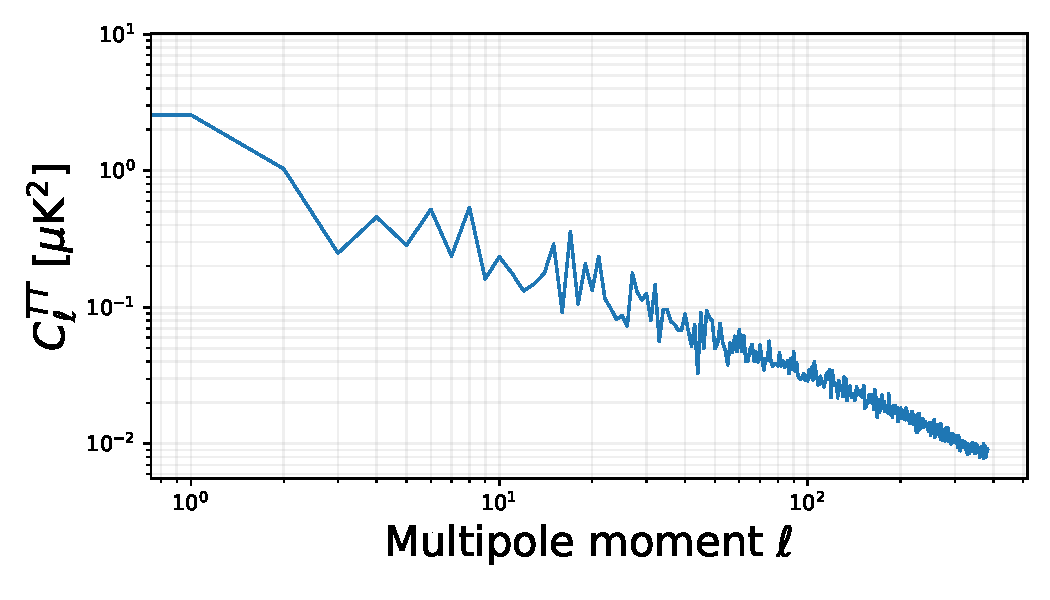
\includegraphics[width=0.9\linewidth]{psTT_lbs.pdf}
    \end{minipage}
    \hfill
    \begin{minipage}{0.48\textwidth}
      \centering
      {\color{mDarkTeal} \scriptsize \textbf{add\_OofaNoise} (Filtri)}\\
      \vspace{0.05cm}
      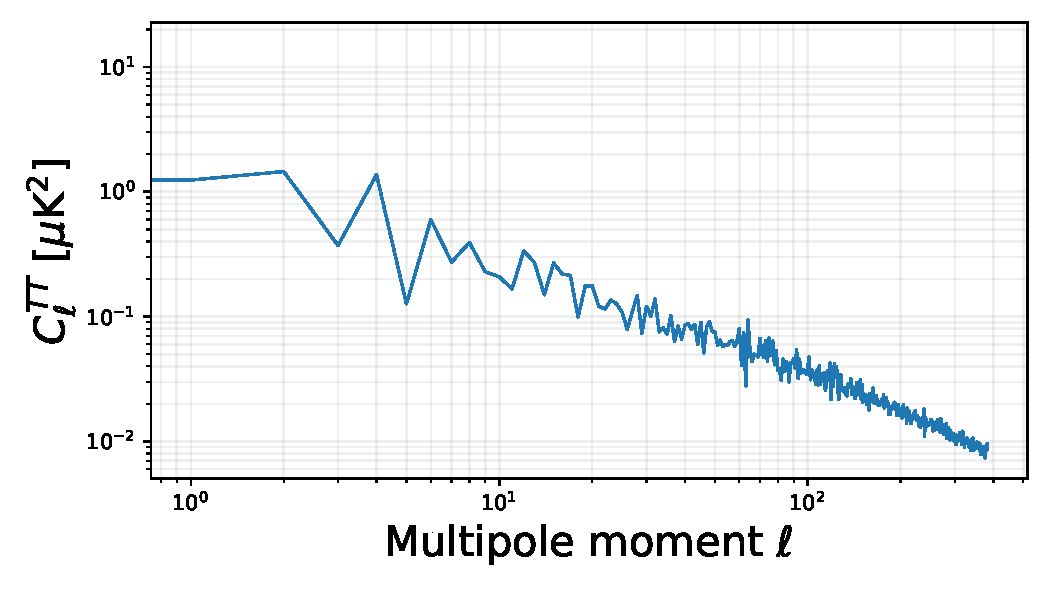
\includegraphics[width=0.9\linewidth]{psTT_oofa.pdf}
    \end{minipage}
  \end{center}

  \vspace{0.1cm}
  {\color{gray!30}\hrulefill}
  \vspace{0.1cm}

  % --- PARTE BASSA: ANALISI CONCETTUALE ---
  \begin{columns}[T]
    \begin{column}{0.5\textwidth}
      \metroset{block=transparent}
      \begin{block}{Corrispondenza PSD $\rightarrow C_\ell$}
        \scriptsize
        Per mappe di solo rumore, l'andamento riflette le proprietà del TOD:
        \centering
        $$C_\ell \propto \left[ 1 + \left( \frac{\ell_{\text{knee}}}{\ell} \right)^\alpha \right]$$
      \end{block}
    \end{column}

    \begin{column}{0.5\textwidth}
      \begin{itemize}
        \item \footnotesize \textbf{Eccesso potenza ai bassi $\ell$.}
        \item \footnotesize \textbf{Assenza plateau bianco a alti $\ell$.}
        \item[] \footnotesize $\rightarrow$ \textit{Evidenza della potenziale contaminazione dei Modi B.}
      \end{itemize}
      \vspace{0.1cm}
      \centering
        \tikz[baseline=(char.base)]{\node[red, font=\bfseries\tiny, draw=red, rounded corners=2pt, inner sep=2pt] (char) {SENZA DESTRIPING};}
    \end{column}
  \end{columns}

\end{frame}




%-------------------------------------------
% SLIDE E: DETTAGLI
%-------------------------------------------
\begin{frame}{Backup: Dettagli Implementativi}
  \begin{columns}[T]
    % --- COLONNA SINISTRA: ALGORITMI ---
    \begin{column}{0.55\textwidth}
      \metroset{block=transparent}
      \begin{block}{Implementazione del Rumore $1/f$}
        \footnotesize
        \begin{itemize}
            \item \textbf{Metodo FFT (\texttt{add\_noise}):}
            Generazione rumore bianco $\rightarrow$ FFT $\rightarrow$ Scaling delle ampiezze secondo la PSD (fasi invariate).
            \item \textbf{Filtri Digitali (\texttt{OofaNoise}):}
            State machine che trasforma input gaussiano attraverso una serie di filtri complessi.
        \end{itemize}
      \end{block}

    \vspace{0.1cm}
    
      \begin{block}{Parallelizzazione}
        \footnotesize
        \begin{itemize}
            \item \textbf{FFT:} Facilmente parallelizzabile (blocchi indipendenti), ma \textbf{discontinua} sulle derive $1/f$.
            \item \textbf{Filtri:} Parallelizzabile per \textbf{detector}. Non parallelizzabile nel tempo (natura ricorsiva), ma preserva la continuità.
        \end{itemize}
      \end{block}
    \end{column}

    % --- COLONNA DESTRA: MEMORIA ---
    \begin{column}{0.4\textwidth}
      \vspace{0.5cm}
      \centering
      \small \textbf{Footprint di Memoria}
      \vspace{0.2cm}
      
      \rowcolors{2}{gray!5}{white}
      \begin{tabular}{ll}
        \toprule
        \textbf{Metodo} & \textbf{RAM} \\
        \midrule
        FFT & $\propto$ Dim. Blocco \\
        Filtri & \textbf{Costante} \\
        \bottomrule
      \end{tabular}
      
      \vspace{0.4cm}
      \begin{exampleblock}{Dettaglio Filtri}
        \scriptsize
        1 Filtro = 5 float64 (40 Byte) \\
        Generatore $1/f$ = 5 Filtri \\
        \textbf{Totale $\approx$ 200 Byte}
      \end{exampleblock}
      
    \end{column}
  \end{columns}
\end{frame}




%-------------------------------------------
% SLIDE F: CONTINUITÀ
%-------------------------------------------
\begin{frame}[fragile]{Backup: Continuità tra Blocchi}
  \metroset{block=transparent}
  
  \begin{columns}[T]
    % --- COLONNA LBS (FFT) ---
    \begin{column}{0.48\textwidth}
      \begin{block}{\texttt{add\_lbsNoise} (FFT)}
        \fontsize{7pt}{8pt}\selectfont
        \begin{itemize}
            \item \textbf{Stateless}: Non ha memoria tra i blocchi.
        \end{itemize}
        \begin{semiverbatim}
\textcolor{gray}{# Loop sui blocchi}
for start in range(0, n_samp, n_block):
    end = min(start + n_block, n_samp)
    
    \textcolor{orange!80!black}{\textbf{lbs.add_noise}}(
        tod=tod[:, start:end],
        \textcolor{gray}{# Funzione chiamata a ogni blocco}
    )
    \textcolor{gray}{# Ogni chiamata genera fasi}
    \textcolor{gray}{# casuali indipendenti.}
        \end{semiverbatim}
        \centering
        \tikz{\node[red, font=\tiny\bfseries, draw=red, rounded corners=2pt] {DISCONTINUITÀ AI BORDI};}
      \end{block}
    \end{column}

    % --- COLONNA FILTRI (OOFA) ---
    \begin{column}{0.48\textwidth}
      \begin{block}{\texttt{add\_OofaNoise} (Filtri)}
        \fontsize{7pt}{8pt}\selectfont
        \begin{itemize}
            \item \textbf{Stateful}: Preserva lo stato del filtro.
        \end{itemize}
        \begin{semiverbatim}
\textcolor{orange!80!black}{\textbf{gens = [OofaNoise(...) for _ in dets]}}
\textcolor{gray}{# Istanza creata FUORI dal loop}

for start in range(0, n_samp, n_block):
    for d in range(n_det):
        \textcolor{gray}{# Il filtro riparte dallo}
        \textcolor{gray}{# stato interno precedente}
        tod[d, start:end] += \\
           \textcolor{orange!80!black}{\textbf{gens[d].filterGaussian}}(...)
        \end{semiverbatim}
        \centering
        \tikz{\node[mDarkTeal, font=\tiny\bfseries, draw=mDarkTeal, rounded corners=2pt] {CONTINUITÀ GARANTITA};}
      \end{block}
    \end{column}
  \end{columns}

\end{frame}





%-------------------------------------------
% SLIDE G: MODI E vs MODI B
%-------------------------------------------
\begin{frame}{Backup: Polarizzazione CMB}

  \begin{columns}[c]
    % --- COLONNA SINISTRA: IMMAGINE ---
    \begin{column}{0.45\textwidth}
      \centering
      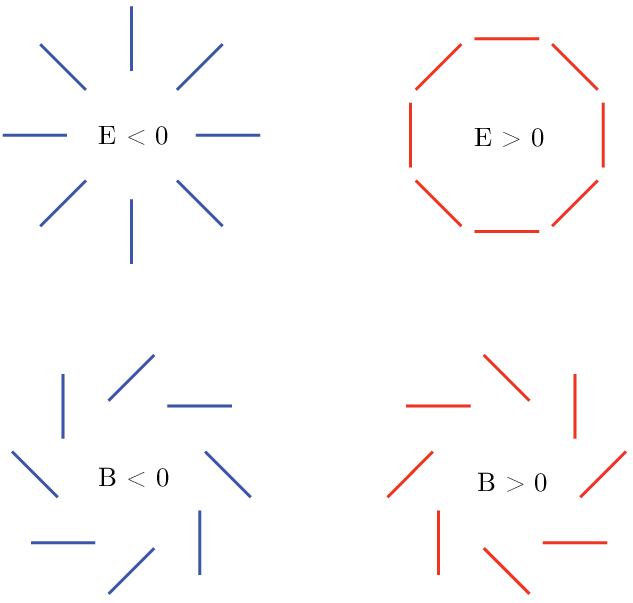
\includegraphics[width=0.85\linewidth]{1_eb_modes.png}
      \vspace{0.2cm}
      \begin{itemize}
        \item[\checkmark] \footnotesize \textbf{Modi E}: Pattern radiali/tangenziali
        \item[\checkmark] \footnotesize \textbf{Modi B}: Pattern a sprirale
      \end{itemize}
    \end{column}

    % --- COLONNA DESTRA: CONFRONTO ---
    \begin{column}{0.5\textwidth}
      \metroset{block=transparent}
      
      \begin{block}{Modi E (Scalari)}
        \footnotesize
        \begin{itemize}
          \item Generati da \textbf{perturbazioni di densità}.
          \item Segnale "forte" ($\approx 5-10\,\mu\text{K}$).
          \item Già mappati con precisione.
        \end{itemize}
      \end{block}

      \begin{block}{Modi B (Tensoriali)}
        \footnotesize
        \begin{itemize}
          \item Generati da \textbf{onde gravitazionali primordiali}.
          \item Segnale "debolissimo" ($\ll 0.1\,\mu\text{K}$).
          \item Prova dell'Inflazione.
        \end{itemize}
      \end{block}

      \vspace{0.1cm}
      \begin{alertblock}{Contaminazioni}
        \fontsize{7pt}{8pt}\selectfont
        \begin{itemize}
          \item \textbf{Lensing Gravitazionale} (conversione $E \rightarrow B$).
          \item \textbf{Foregrounds Galattici} (polvere e sincrotrone).
          \item \textbf{Rumore Strumentale}.
        \end{itemize}
      \end{alertblock}
    \end{column}
  \end{columns}

\end{frame}



%-------------------------------------------
% SLIDE H: DETECTOR
%-------------------------------------------
\begin{frame}{Backup: Detector di LiteBIRD}
    \metroset{block=transparent}
    \footnotesize % Font leggermente ridotto per far respirare la slide

    % --- BLOCCO 1: FISICA ---
    \begin{block}{Bolometro come Calorimetro}
        $\rightarrow$ Misura il \textbf{flusso} della radiazione, che induce una variazione di temperatura.
        \vspace{-0.2cm}
        \begin{itemize}
            \item CMB $=$ spettro di Corpo Nero $\rightarrow$ Data una banda di frequenze, posso ricostruire lo spettro di Planck attraverso l'associazione biunivoca tra flusso misurato e temperatura.
        \end{itemize}
    \end{block}

    \vspace{0.1cm}

    % --- BLOCCO 2: SELEZIONE ---
    \begin{block}{Assorbimento e Selezione}
        $\rightarrow$ Il bolometro \textbf{non discrimina} frequenza, assorbe tutto (corpo nero). Se riflettesse il fotone:
        \vspace{-0.2cm}
        \begin{enumerate}
            \item Mancata misura (perdita statistica).
            \item Assorbimento da parte di altri detector (effetti sistematici).
        \end{enumerate}
        \vspace{-0.2cm}
        \begin{itemize}
            \item \textbf{Horn} (Antenna): Seleziona radiazione all'interno della banda di frequenza (\textit{bandwidth} $\approx 20\%$).
        \end{itemize}
    \end{block}

    \vspace{0.1cm}

    % --- BLOCCO 3: POLARIZZAZIONE ---
    \begin{block}{Misura della Polarizzazione}
        $\rightarrow$ Il design attuale (non ancora definito) prevede due soluzioni:
        \vspace{-0.2cm}
        \begin{itemize}
            \item \textbf{HWP (Half-Wave Plate):} Modulatore di polarizzazione rotante (scelta preferita).
            \item \textbf{Filtri Polarizzanti:} Griglie che selezionano una sola componente del campo.
        \end{itemize}
    \end{block}

\end{frame}




 




\end{document}
